En esta sección se va a detallar los principales ataques sobre Active Directory y su experimentación en el laboratorio previamente creado. En primer lugar se va a definir en qué consiste dichos ataques y qué debilidad de los protocolos de autenticación utilizan y posteriormente se llevará a cabo una réplica de este ataque en el Active Directory {\it laboratoy.com}. \\

Para la experimentación se da por hecho que el atacante ya ha comprometido el sistema Cliente01 a través de cualquier técnica de explotación y ha conseguido escalar privilegios y dispone de una {\it Reverse Shell} interactiva. A partir de este supuesto, se rea\-li\-za\-rá movimientos laterales y/o verticales a través del Active Directory. También se asume que las herramientas utilizadas están ofuscadas y eluden las protecciones de antivirus que pueda tener el sistema comprometido al no presentarse en el alcance ni los objetivos de este proyecto.

\section{Pass the hash}

La idea principal del ataque {\it Pass the hash (PtH)}~\cite{Capitulo5:PtHMitre} es la autenticación de un usuario legítimo sin la necesidad de conocer la contraseña de usuario en texto claro. Para ello, el atacante únicamente debe disponer del hash de la contraseña del usuario a suplantar. Los inicios de este ataque o técnica de movimiento lateral se retoman a 1997 cuando Paul Ashton lanzó el primer {\it Pass the hash (PtH)} con una versión de SMB modificado~\cite{Capitulo5:Paul}.\\

Como se ha observado en los capítulos previos, cuando un usuario se autentica a través del paquete de autenticación NTLM, para su autenticación el cliente cifra un secreto o nonce compartido por el servidor con el Hash NT del usuario~\cite{Capitulo5:HackingWindows}, por lo tanto, no es necesario conocer la contraseña en claro. Además, los hashes del usuario se mantienen en la memoria (a través del proceso LSASS) lo que permite que, una vez autenticado un usuario legítimo, cuando el sistema requiera otra autenticación para acceder a un recurso se haga de manera trasparente al usuario.\\ 

Por lo tanto, para llevar a cabo esta técnica, es necesario que el atacante obtenga el Hash NT del usuario al que quiera suplantar. Este hash puede ser obtenido a través del volcado de la base de datos SAM \footnote{C:\textbackslash{}windows\textbackslash{}system32\textbackslash{}config\textbackslash{}SAM}, de copias de seguridad o {\it backups} de esta \footnote{C:\textbackslash{}windows\textbackslash{}repair\textbackslash{}sam}, el volcado de las credenciales almacenadas por el usuario en el proceso LSASS (tiene que haber una logonsession con dicho usuario), a través del volcado de credenciales de la base de datos NTDS  o a través de interceptar los mensajes {\it Challenge-Response} cuando se autentica un usuario y crackeado el Hash NTLM para llegar a sacar el hash NT~\cite{Capitulo5:PtH}. \\

Como abstracción de la capacidad de este ataque, se puede decir que {\it Pass the hash (PtH)} permite de manera efectiva la suplantación de cualquier empleado o cliente de una empresa, sin la necesidad de conocer la contraseña, únicamente conociendo el Hash NT de esta. Por lo tanto, el uso de contraseñas robustas no protegería de este tipo de ataques. \\

\subsubsection{Experimentación}

Una vez obtenido una {\it Reverse Shell} interactiva con privilegios de administrador se va a realizar la técnica de {\it Pass The Hash} a través del usuario administrador {\it federicogar}. Este usuario se ha logueado previamente en el Cliente01 por lo tanto tiene una logon session en la máquina. 

\begin{enumerate}
\item Se obtiene la {\it Reverse Shell} interactiva en la máquina atacante. Se ejecuta el comando {\it whoami} y vemos que somos el usuario de dominio {\it LABORATORY\textbackslash{}mariarperez} y no se tienen privilegios suficientes para listar el directior {\it C\$} de la máquina DC01 (Figura \ref{PTH1}).
\begin{figure}[H] %[ht!] para here [b] para bottom [t] para top
\begin{center}
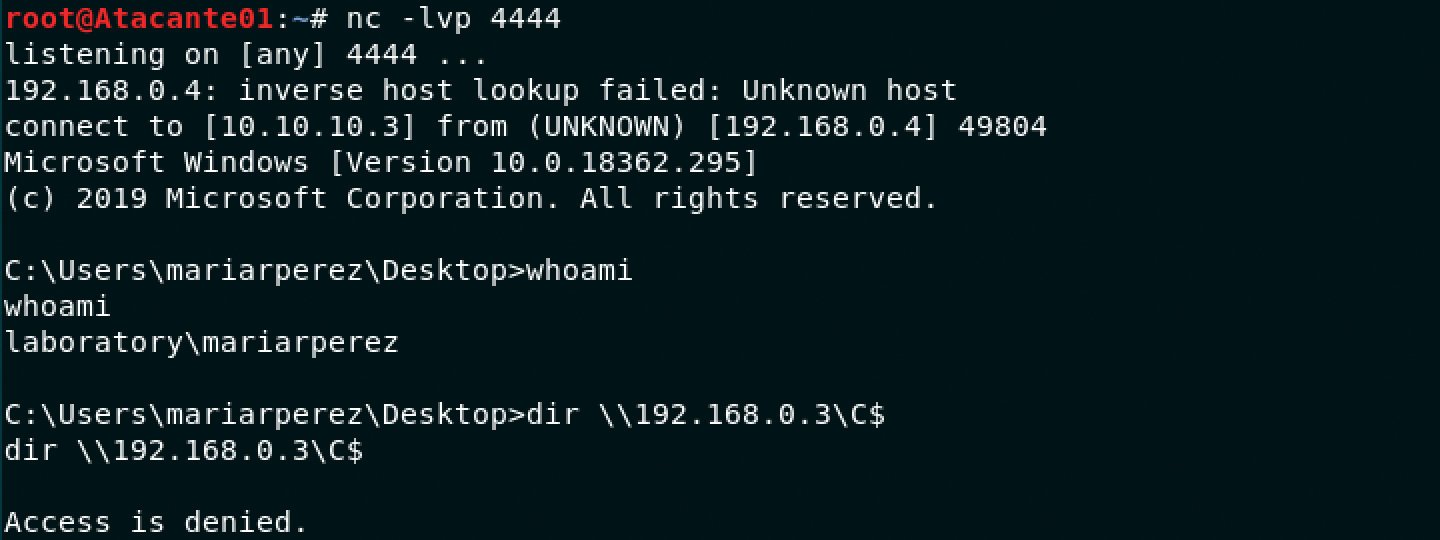
\includegraphics[width=15cm]{PTH/PTH1.png}
\end{center}
\caption{Reverse Shell interactiva sin privilegios.}
\label{PTH1}
\end{figure}

\item Si se recoge el tráfico intercambiado entre la máquina Cliente01 y el DC01, se puede ver que al intentar listar un directorio a través de la IP de éste se realiza a través del protocolo SMB utilizando el protocolo de autenticación NTLM donde el user es {\it LABORATORY\textbackslash{}mariarperez}. Al no tener privilegios, se ha denegado el acceso (Figura \ref{PTH2}).
\begin{figure}[H] %[ht!] para here [b] para bottom [t] para top
\begin{center}
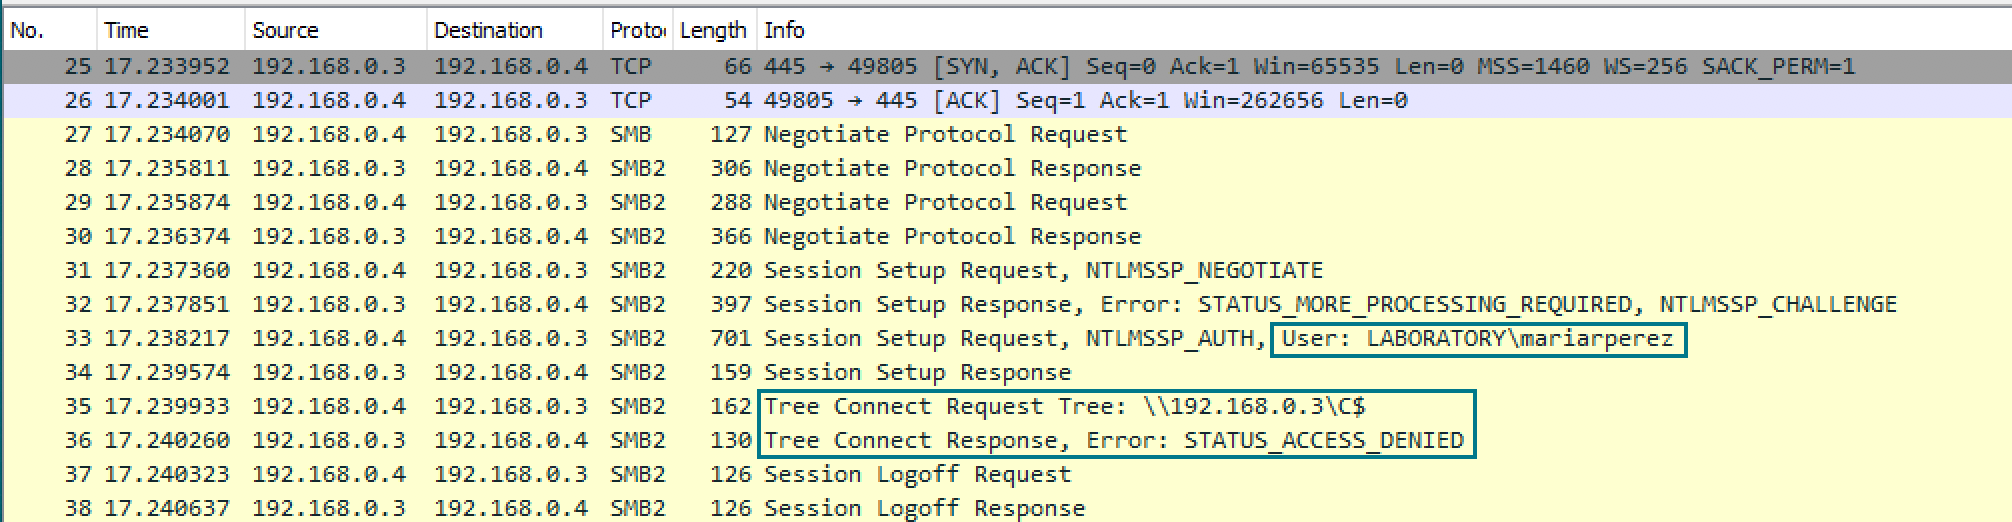
\includegraphics[width=15cm]{PTH/PTH2.png}
\end{center}
\caption{Paquetes intercambiados entre Cliente01 y DC01 - Sin pass the hash.}
\label{PTH2}
\end{figure}

\item  Al disponer de una sesión válida el usuario {\it federicogar} se puede  obtener el hash de la contraseña del proceso LSASS. Para ello, se ha utilizado la herramienta Mimikatz~\cite{Capitulo5:Mimikatz} a través de los siguientes comandos (Figura \ref{PTH3}).
\begin{listing}[style=consola, numbers=none]
# privilege::debug
# sekurlsa::logonpasswords
\end{listing}

\begin{figure}[H] %[ht!] para here [b] para bottom [t] para top
\begin{center}
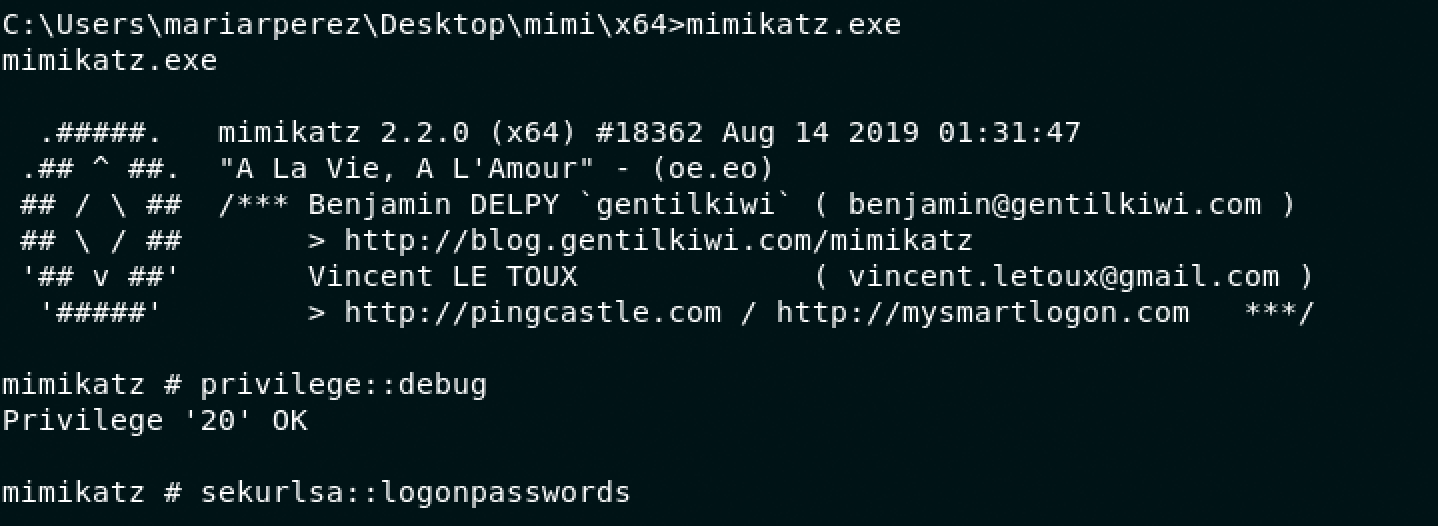
\includegraphics[width=15cm]{PTH/PTH3.png}
\end{center}
\caption{Comandos Mimikatz para listas sesiones activas.}
\label{PTH3}
\end{figure}

\item El comando anterior lista todas las sesiones activas en el usuario, por lo tanto, se busca la que pertenece al usuario víctima y se obtiene el Hash NT (Figura \ref{PTH4}).
\begin{figure}[H] %[ht!] para here [b] para bottom [t] para top
\begin{center}
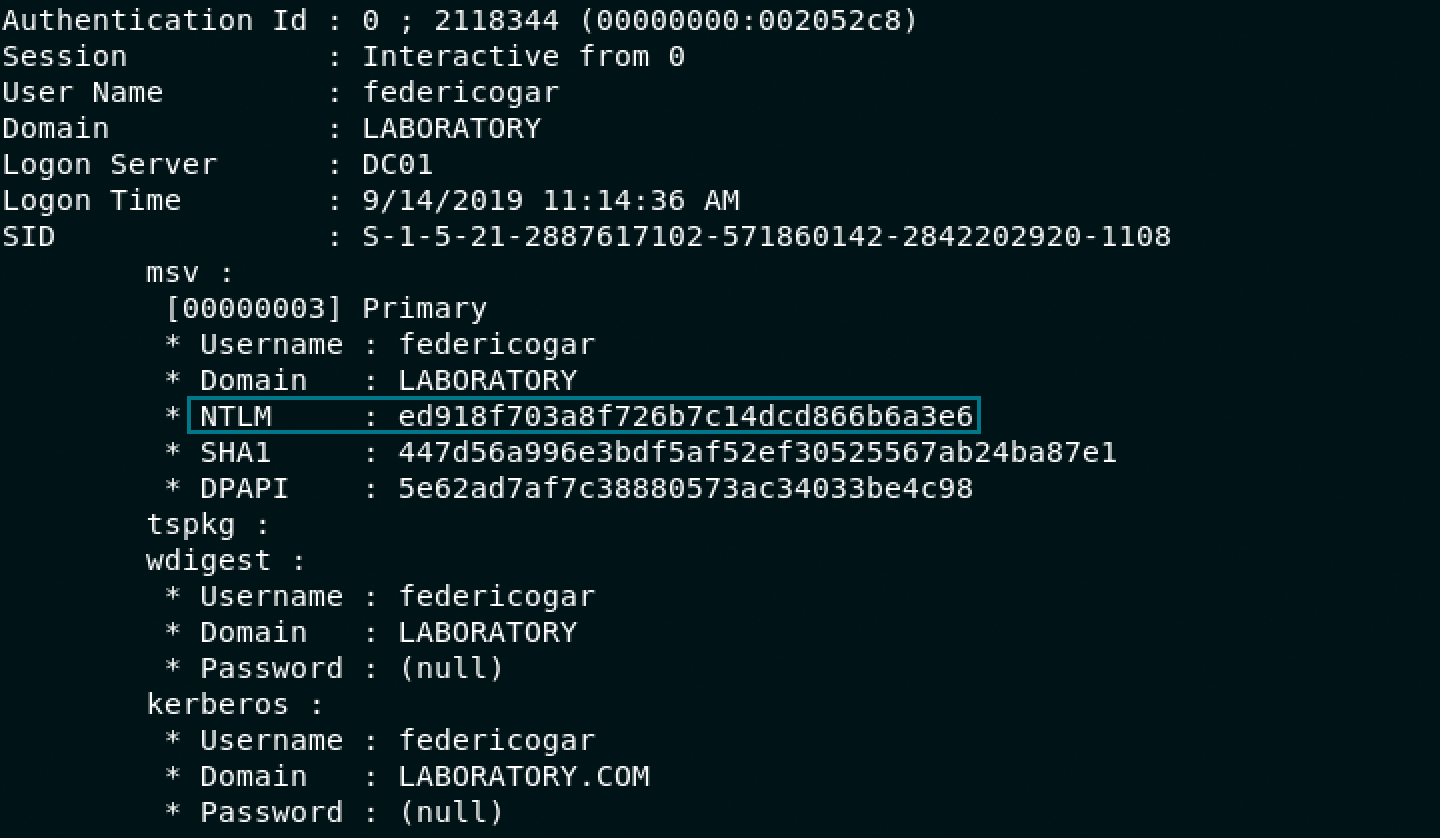
\includegraphics[width=15cm]{PTH/PTH4.png}
\end{center}
\caption{Hash del usuario víctima.}
\label{PTH4}
\end{figure}

\item La propia herramienta Mimikatz permite realizar el ataque Pass the Hash a través del siguiente comando, el resultado de este comando se puede observar en la Figura \ref{PTH5}.
\begin{listing}[style=consola, numbers=none]
# sekurlsa::pth /user:federicogar /ntlm:ed918f703a8f726b7c14dcd866b6a3e6 /domain:LABORATORY /run:cmd.exe
\end{listing}


\begin{figure}[H] %[ht!] para here [b] para bottom [t] para top
\begin{center}
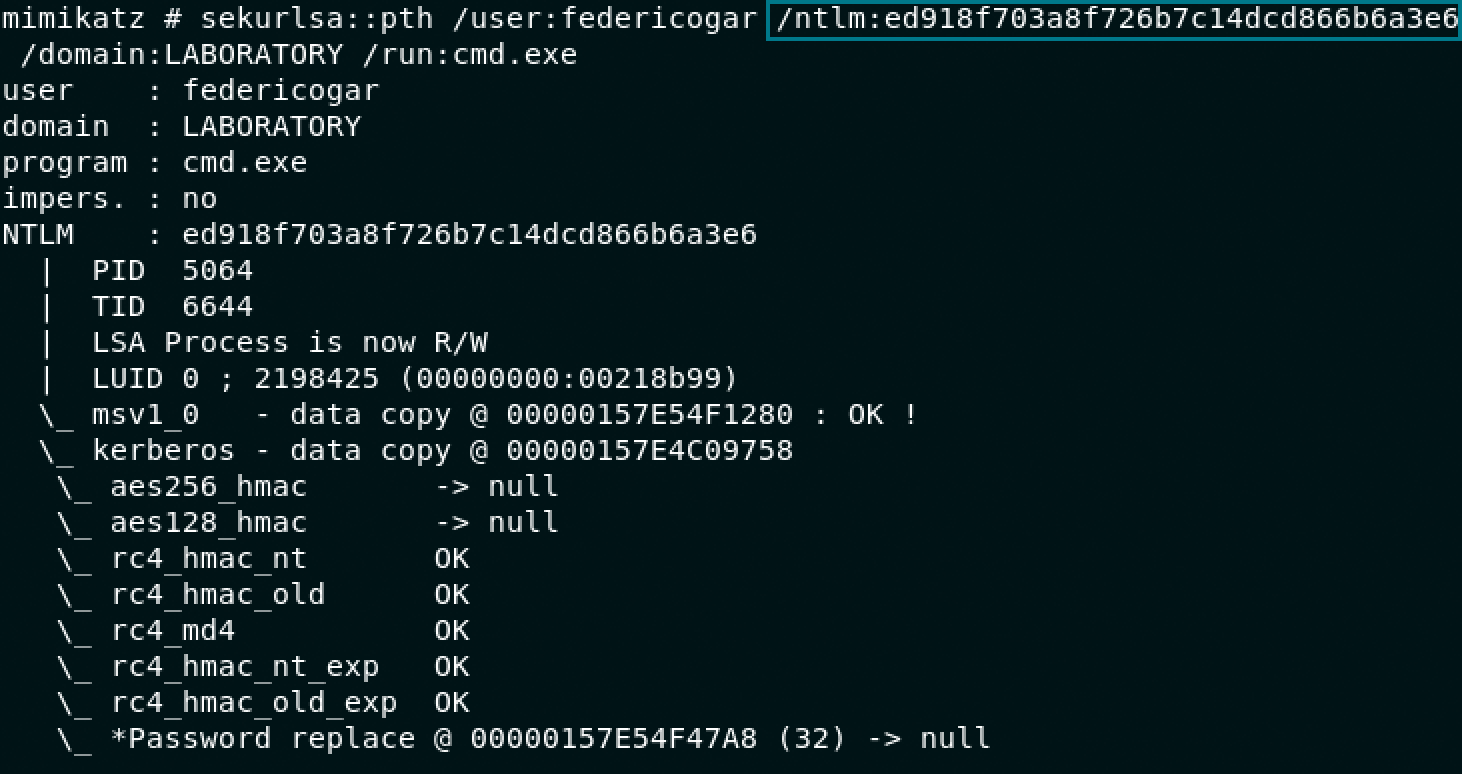
\includegraphics[width=15cm]{PTH/PTH5.png}
\end{center}
\caption{Pash the hash a través de la herramienta Mimikatz.}
\label{PTH5}
\end{figure}

\item En el comando anterior, se definió ejecutar el comando {\it cmd.exe}. Este comando se ejecutará en el Cliente01, por lo tanto, si queremos que se ejecute otra {\it Reverse Shell} con privilegios del usario víctima sería necesario especificar otro comando. En la shell resultante (Figura \ref{PTH6}) se puede observar que aunque seguimos siendo el usario {\it mariarperez} se puede listar los archivos de DC01. Esto es debido a que Mimikatz genera una nueva sesión para el usuario {\it mariarperez} y sobreescribe el contenido de las credenciales con el hash del otro usuario. 
\begin{figure}[H] %[ht!] para here [b] para bottom [t] para top
\begin{center}
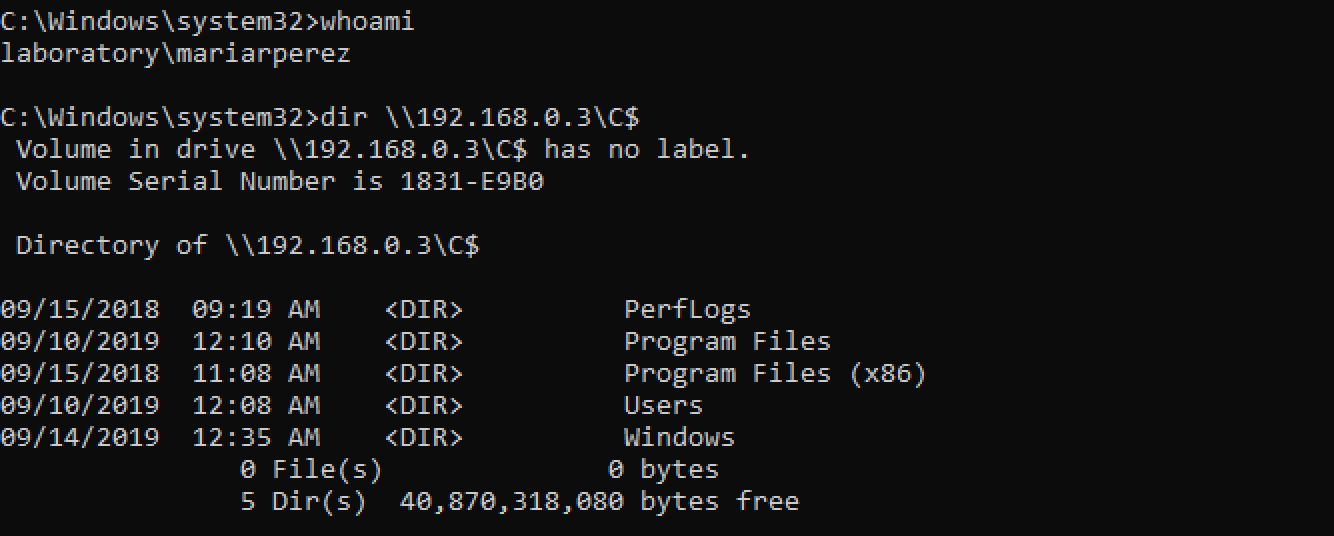
\includegraphics[width=15cm]{PTH/PTH6.png}
\end{center}
\caption{Ataque pass the hash realizado correctamente.}
\label{PTH6}
\end{figure}

\item Por último, al recoger el tráfico generado en esta comunicación se puede observar bastantes diferencias con la figura anterior. Ahora el usuario es {\it federicogar} y se ha realizado el {\it Challenge-Response} de NTLM satisfactoriamente pudiendo listar los ficheros (Figura \ref{PTH7}).
\begin{figure}[H] %[ht!] para here [b] para bottom [t] para top
\begin{center}
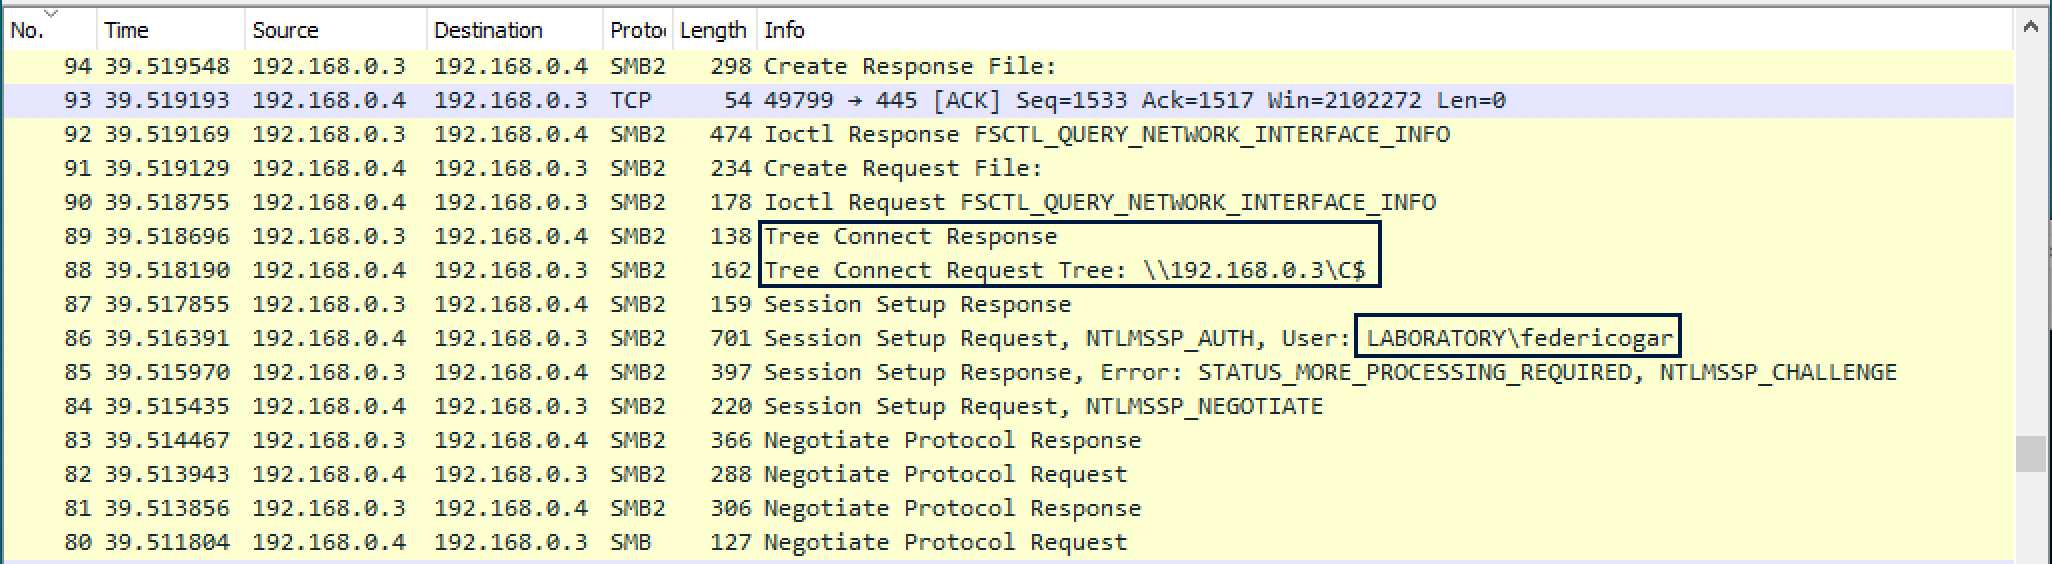
\includegraphics[width=15cm]{PTH/PTH7.png}
\end{center}
\caption{Paquetes intercambiados entre Cliente01 y DC01 - Con pass the hash.}
\label{PTH7}
\end{figure}

\end{enumerate}

\section{NTLM Relay}

Hoy en día los ataques de {\it NTLM Relay} son un técnica muy utilizada por {\it Pentesters} y atacantes permitiendo el acceso a activos o recursos críticos incluso si la organización dispone de buenas prácticas para la gestión de la seguridad. A grandes rasgos, esta técnica de movimiento lateral o vertical se puede sintetizar como un ataque de {\it pass the hash} pero a nivel de red. \\ 


Para entender este ataque es necesario entender el protocolo {\it Challenge - Respuesta} utilizado por NTLM. Aunque se ha detallado anteriormente se puede sintetizar en las siguientes fases: 

\begin{enumerate}
\item El cliente intenta iniciar sesión en un servicio o recurso.
\item El servidor responde con un desafío o {\it challenge}, es decir, el cliente dice, si eres quién dice ser, cifra este desafío con tu hash de la contraseña.
\item El cliente cifra el desafío.
\item El servidor compueba la validez de este paquete, descifrando  el desafio ya que dispone del hash del usuario. Si es correcto, verifica al usuario. 
\end{enumerate}

En un ataque de NTLM Relay, el atacante se sitúa como intermediario entre los paquetes intercambiados en el proceso anterior. Para ello, selecciona el recurso o activo en el que quiere autenticarse y espera a que un usuario legítimo intente conectarse a él. A continuación, se va a detallar cómo cambia el esquema de autenticación NTLM cuando se está produciendo un ataque de {\it NTLM Relay}~\cite{Capitulo5:NTLMRelay}:

\begin{enumerate}
\item En primer lugar, el cliente intenta conectarse a un recurso. Esta petición es interceptada por un atacante y reenviada al servidor objetivo. 
\item El servidor contesta con un desafío, este desafío también es interceptado por el atacante y reenviado a la víctima.
\item La víctima cifra con el Hash NT de la contraseña el desafío y crea un paquete que será enviado de nuevo al atacante y este lo reenviará al servidor. 
\item El servidor comprueba que el desafío se ha cifrado correctamente y concede el acceso a dicho recurso. Por lo tanto, el atacante tiene acceso a ese recurso ya que dispone del paquete con el desafío cifrado. 
\item Por último, el atacante manda un paquete a la víctima denegando el acceso a ese recurso. 
\end{enumerate}

Como es de esperar, este tipo de ataques han sido perseguidos de cerca por Microsoft y ha implementado medidas que dificultan o imposibilitan este ataque. Una de ellas es el parche MS08-068~\cite{Capitulo5:MS08-068} que imposibilita que se pueda retrasmitir un Hash NTLM a la misma máquina de la que se obtuvo imposibilitando así los ataques de NTLM Replay reflejado. Sin embargo, estos hashes se pueden retrasmitir a otros servicios o máquinas. \\

Para replicar este tipo de ataques en el laboratorio local se va a utilizar la herramienta Responder~\cite{Capitulo5:Responder}. Antes de definir esta herramienta es necesario hablar de los {\it Windows Name Resolution}, es decir, de la forma que utilizada Microsoft para resolver los nombres de dominio. Para ello, se utilizan los protocolos: {\it Link Local Multicast Name Resolution (LLMNR)} y {\it NetBIOS over TCP/IP Name Service}. La herramienta Responder realiza un ``envenenamiento'' de estos protocolos y permite obtener las credenciales en red. Esta herramienta crea servidores de autenticación como puede ser SMB, MYSQL, HTTP(s), FTP... y obliga a la víctima a enviar las credenciales a estos servidores y así poder obtenerlas. \\

Por lo tanto, con la herramienta Responder se puede obtener los Hashes NTLM de una conexión de autenticación y retrasmitirlos a través de otra herramienta como puede ser {\it ntlmrelayx.py} de la librería de Impacket o {\it MultiRelay.py}. \\

Una de las limitaciones de este ataque es que la medida que implementó Windows: SMB Signing~\cite{Capitulo5:SMBSigning} debe estar desactivada. Esta medida firma los paquetes SMB para evitar que estos sean modificados durante su retrasmisión. Se puede suponer que esta medida esta desactivada ya que en la mayoría de los Sistemas Windows están desactivadas a excepción de Windows Server como se puede ver en la Figura \ref{NTLMRelay1}.

\begin{figure}[H] %[ht!] para here [b] para bottom [t] para top
\begin{center}
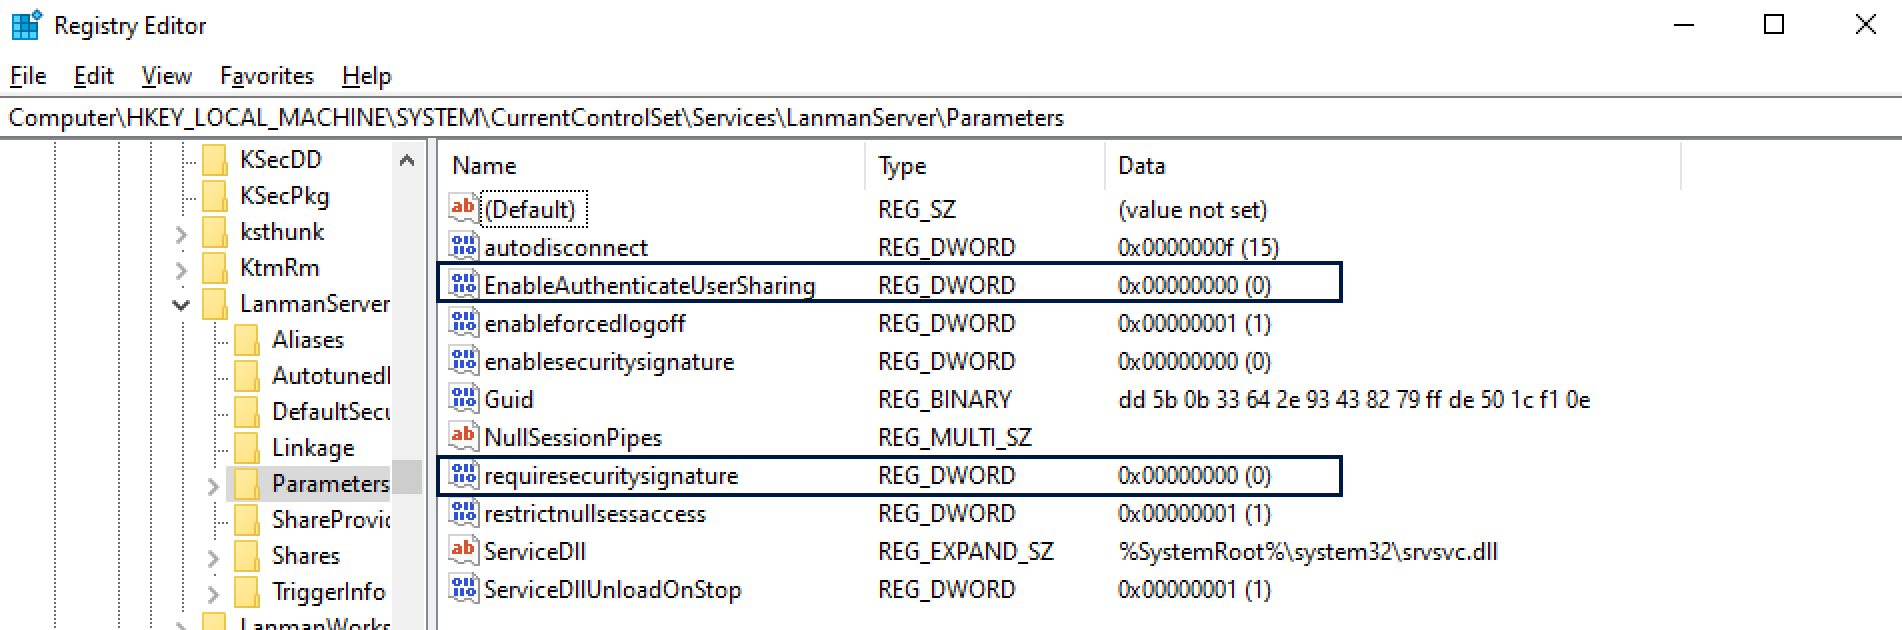
\includegraphics[width=15cm]{NTLMRelay/NTLMRelay1.png}
\end{center}
\caption{SMB Signing desactivado por defecto en Cliente01.}
\label{NTLMRelay1}
\end{figure}

\subsubsection{Experimentación}

Para ejecutar este ataque, la máquina Atacante01 tiene que estar en la misma red. Para ello, desde VirtualBox añadimos una nueva tarjeta de red que esté conectada a ADNET y le asignamos la dirección IP: 192.168.0.5.

\begin{enumerate}

\item En primer lugar, se descarga la última versión de Responder de ~\cite{Capitulo5:Responder} o se utiliza la versión que trae por defecto Kali Linux. En cualquier caso se debe editar el archivo {\it Responder.conf} y deshabilitar las opciones SMB y HTTP para que estas peticiones sean recogidas por {\it ntlmrelayx.py} (Figura \ref{NTLMRelay2}).
\begin{figure}[H] %[ht!] para here [b] para bottom [t] para top
\begin{center}
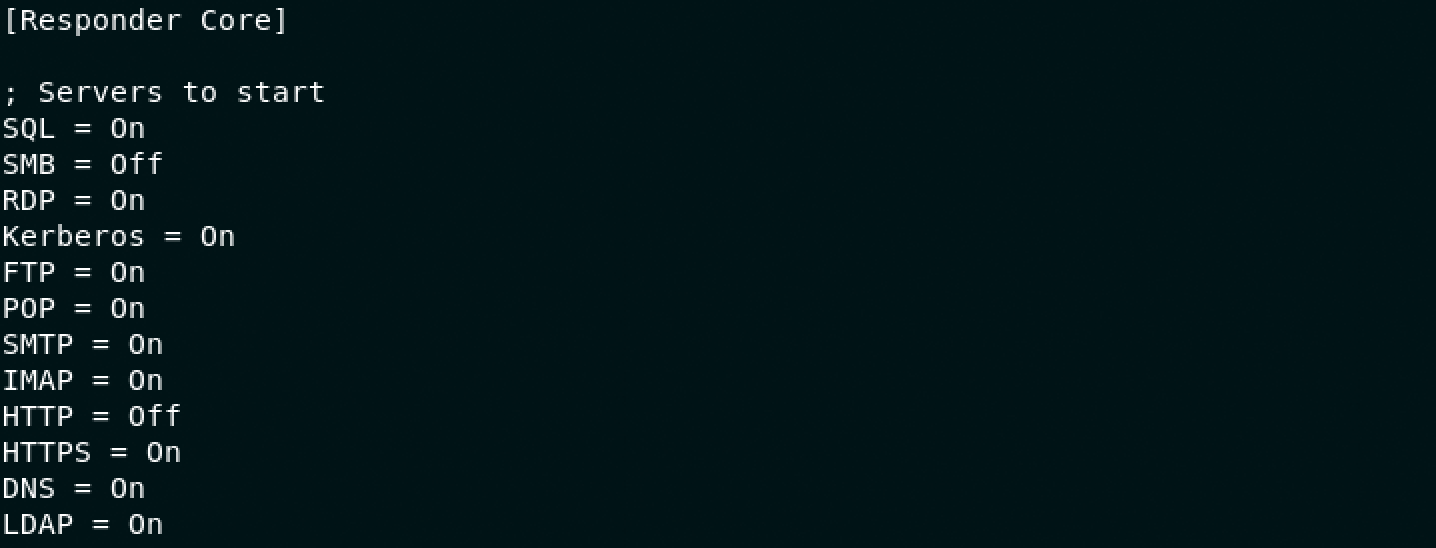
\includegraphics[width=15cm]{NTLMRelay/NTLMRelay2.png}
\end{center}
\caption{Archivo de configuración Responder.conf.}
\label{NTLMRelay2}
\end{figure}

\item Una vez editada la configuración se ejecuta el Responder. En paralelo en otra terminal se ejecuta el {\it ntlmrelayx.py} (Figura \ref{NTLMRelay3}) a través de los siguientes comandos:

\begin{listing}[style=consola, numbers=none]
# .\Responder.py -I eth2 -w -r -f -v
# ntlmrelayx.py -t 192.168.0.3 -smb2support
\end{listing}

-I eth2 - Corresponde a la interfaz de red conectada a la ADNET. \\
-t 192.168.0.3 - Corresponde al target, en este caso DC01. 

\begin{figure}[H] %[ht!] para here [b] para bottom [t] para top
\begin{center}
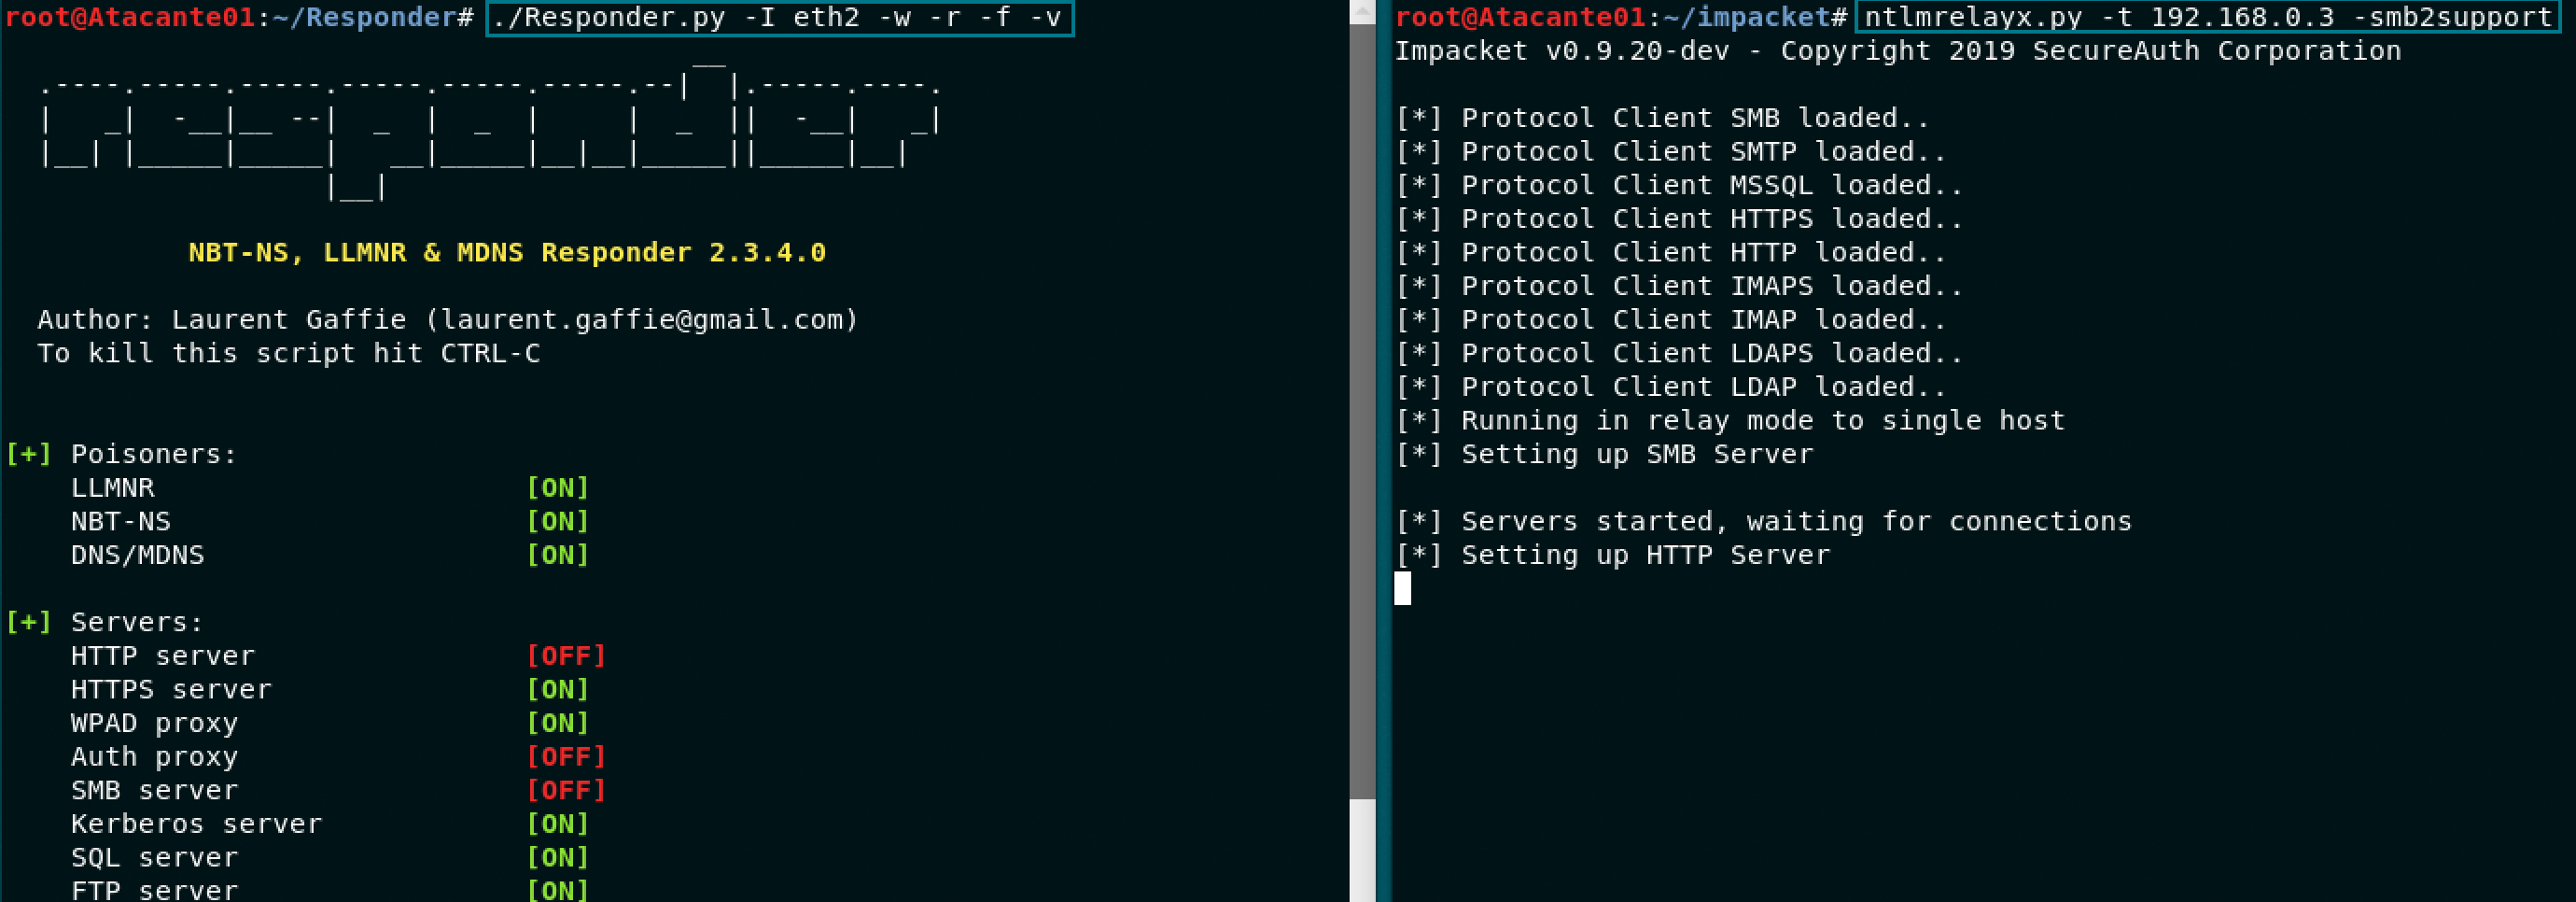
\includegraphics[width=15cm]{NTLMRelay/NTLMRelay3.png}
\end{center}
\caption{Responder y ntlmrelayx.py.}
\label{NTLMRelay3}
\end{figure}

\item Para que este ataque funcione se necesita la interacción del usuario víctima. En este caso bastaría que el usuario con privilegios de Domain Admin se conectara a un recurso inexistente como puede ser \footnote{\textbackslash{}\textbackslash{}test\textbackslash{}C\$} (Figura \ref{NTLMRelay4}).
\begin{figure}[H] %[ht!] para here [b] para bottom [t] para top
\begin{center}
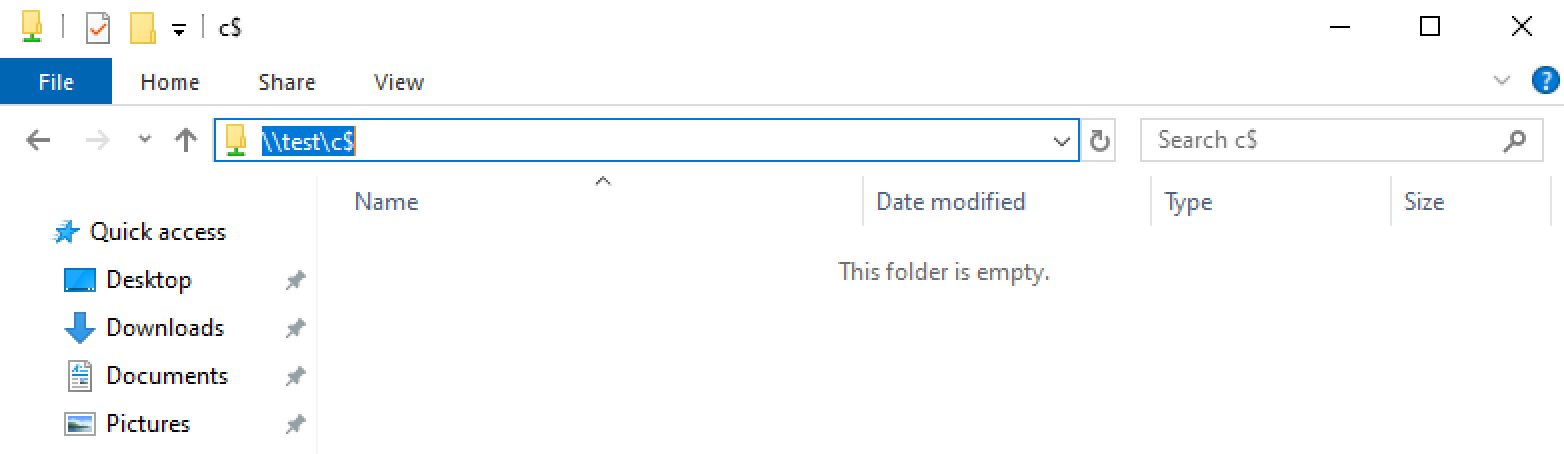
\includegraphics[width=15cm]{NTLMRelay/NTLMRelay4.png}
\end{center}
\caption{Interacción del usuario.}
\label{NTLMRelay4}
\end{figure}

\item Como se puede ver en la Figura \ref{NTLMRelay5} el ataque se ejecuta correctamente y se vuelcan los datos de la SAM del Domain Controller. 
\begin{figure}[H] %[ht!] para here [b] para bottom [t] para top
\begin{center}
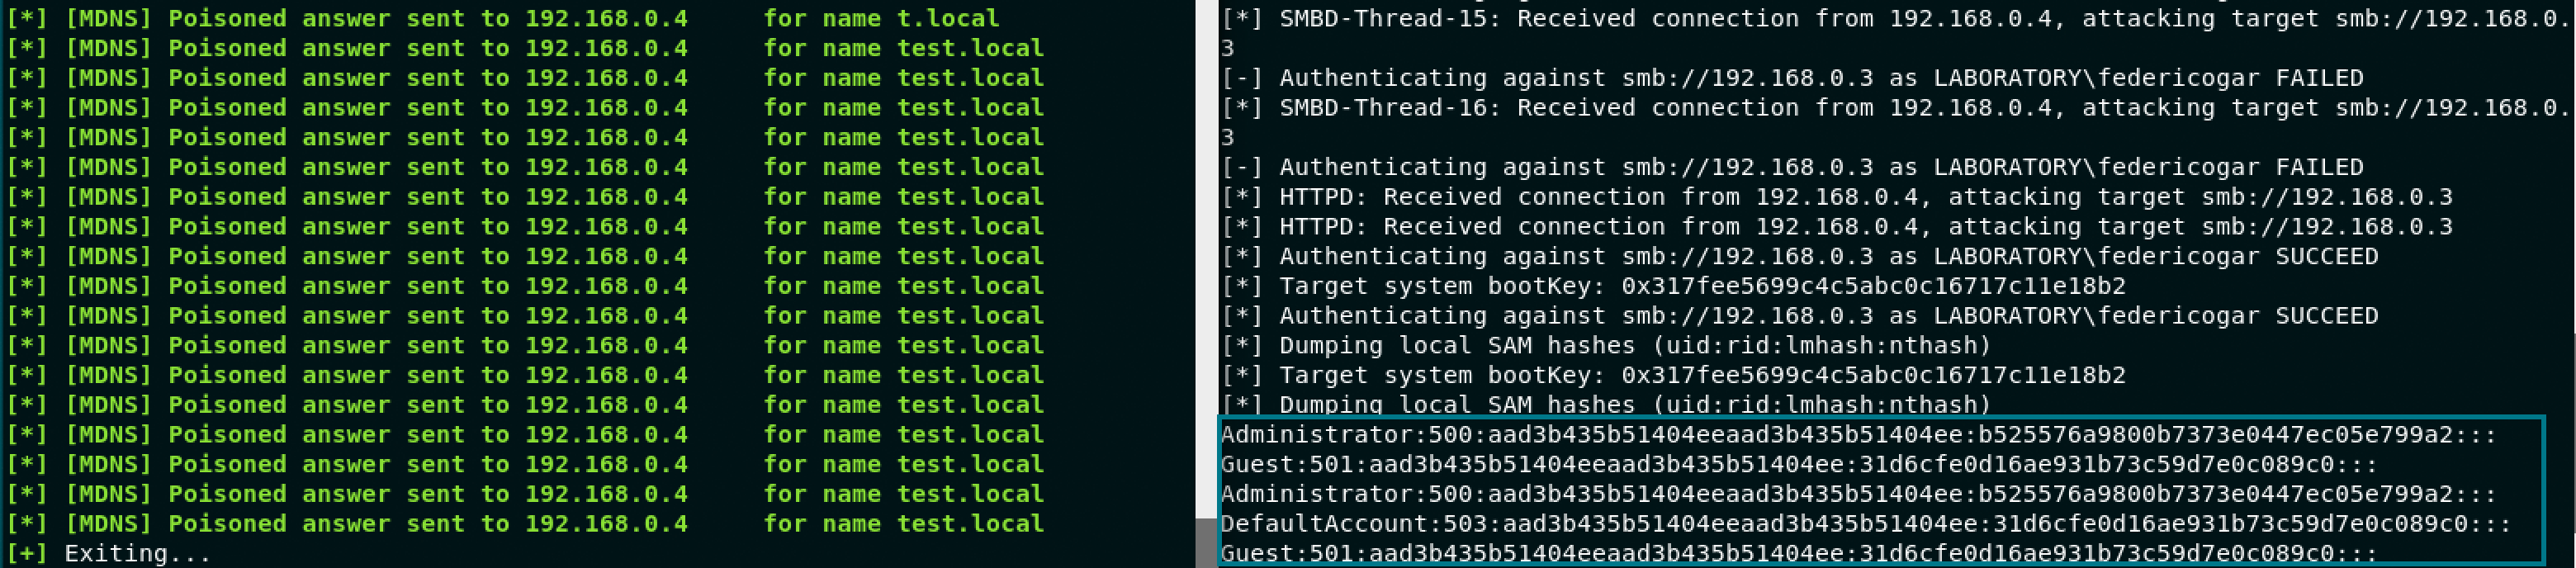
\includegraphics[width=15cm]{NTLMRelay/NTLMRelay5.png}
\end{center}
\caption{Volcado de la SAM.}
\label{NTLMRelay5}
\end{figure}

\end{enumerate}

\section{Overpass The Hash}

La técnica {\it Overpass the hash}, también conocida como {\it Pass the key (PTK)}, es la equivalencia a {\it Pass the hash} para el protocolo de autenticación Kerberos. Como se ha visto anteriormente, durante el intercambio de paquetes, el usuario cifra una marca de tiempo o {\it timestamp}. En función de la versión de Kerberos se va a utilizar un secreto u otro, en este caso en las versiones más antiguas utiliza un secreto RC4 que equivale al Hash NT del usuario, y en versiones más modernas utiliza claves de AES128 y AES256. Por lo tanto, con el Hash NT del usuario se puede obtener un Ticket TGT y  realizar la autenticación correctamente.

\subsubsection{Experimentación}

\begin{enumerate}
\item En primer lugar, se parte desde una {\it Reverse Shell} interactiva con privilegios de administrador del usuario {\it mariarperez} y se trata de listar el directorio {\it C\$} del DC01 a través de protocolo de Kerberos (Figura \ref{OTH1}).
\begin{figure}[H] %[ht!] para here [b] para bottom [t] para top
\begin{center}
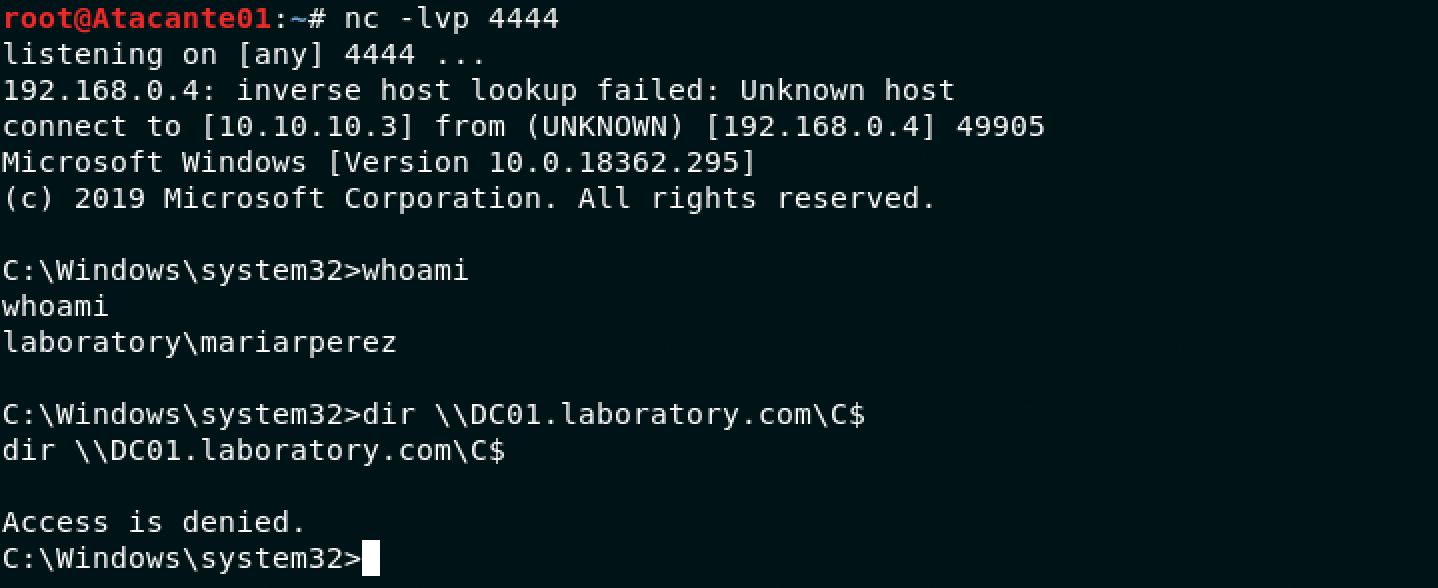
\includegraphics[width=15cm]{OTH/OTH1.png}
\end{center}
\caption{Reverse Shell interactiva.}
\label{OTH1}
\end{figure}

\item Como se puede ver en Wireshark, el intercambio de paquetes KRB5 falla (Figura \ref{OTH2}).
\begin{figure}[H] %[ht!] para here [b] para bottom [t] para top
\begin{center}
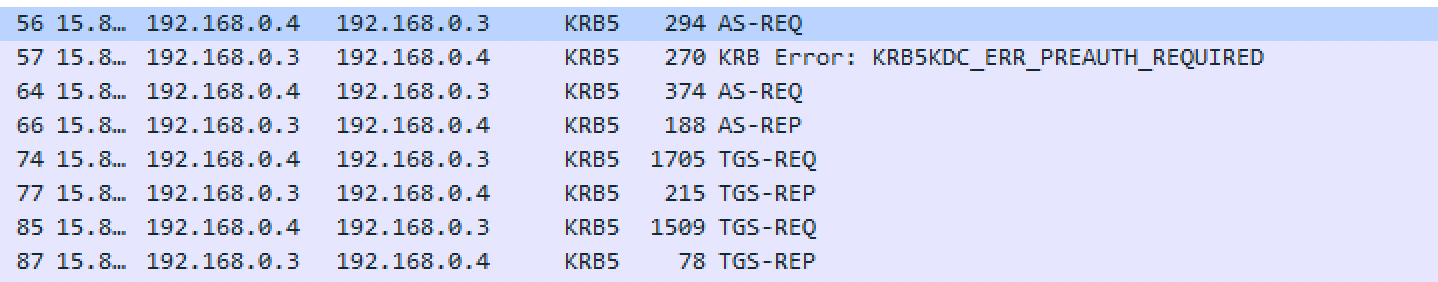
\includegraphics[width=15cm]{OTH/OTH2.png}
\end{center}
\caption{Intercambio de paquetes de Kerberos.}
\label{OTH2}
\end{figure}

\item Se repiten los pasos hechos en {\it Pass the hash} listando las sesiones activas y obteniendo el hash de la contraseña (Figura \ref{OTH3} y Figura \ref{OTH4}).
\begin{figure}[H] %[ht!] para here [b] para bottom [t] para top
\begin{center}
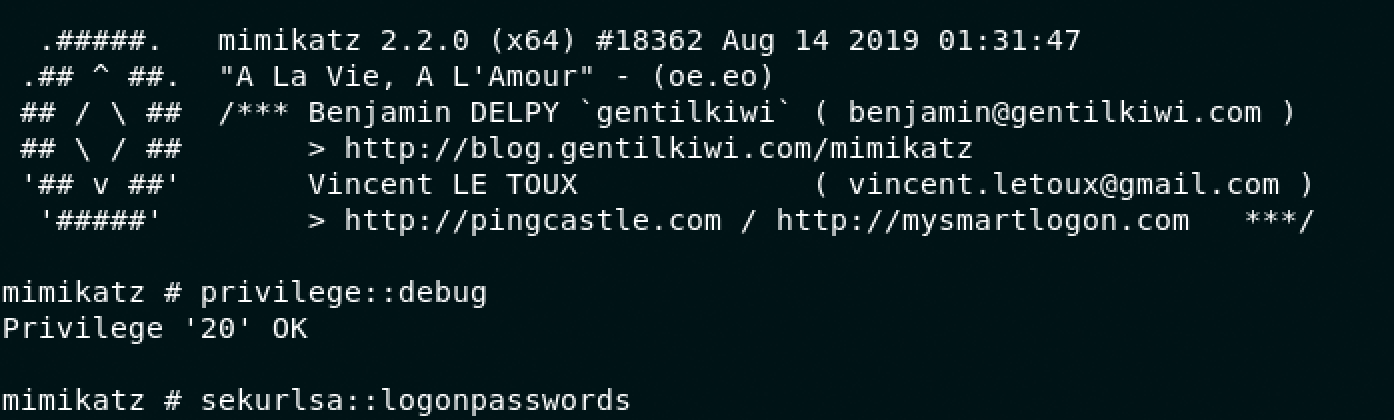
\includegraphics[width=15cm]{OTH/OTH3.png}
\end{center}
\caption{Comandos Mimikatz para listar sesiones activas.}
\label{OTH3}
\end{figure}

\begin{figure}[H] %[ht!] para here [b] para bottom [t] para top
\begin{center}
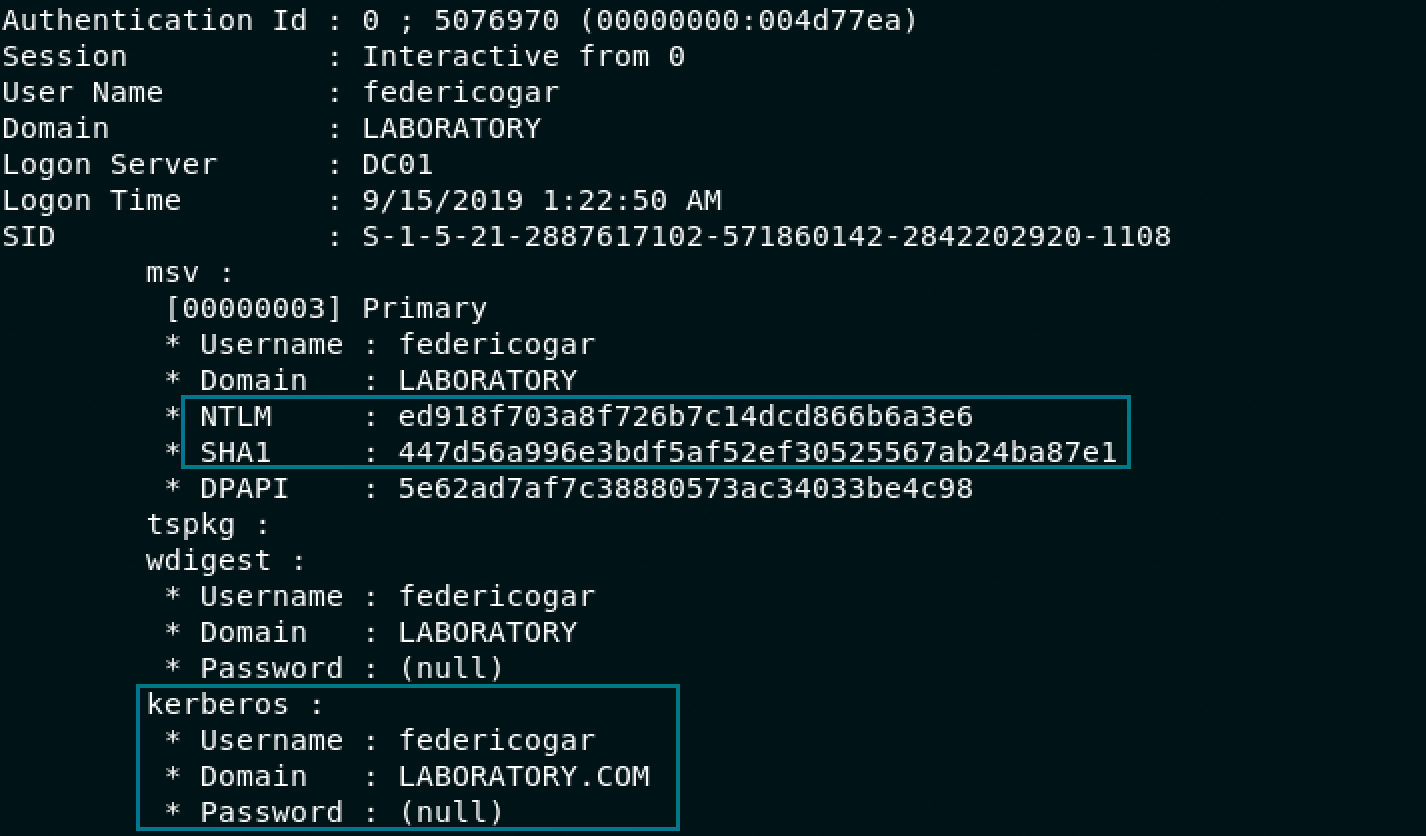
\includegraphics[width=15cm]{OTH/OTH4.png}
\end{center}
\caption{Hash del usario víctima.}
\label{OTH4}
\end{figure}

\item Se realiza el ataque a través del mismo comando que en {\it Pass the hash} (Figura \ref{OTH5}).
\begin{figure}[H] %[ht!] para here [b] para bottom [t] para top
\begin{center}
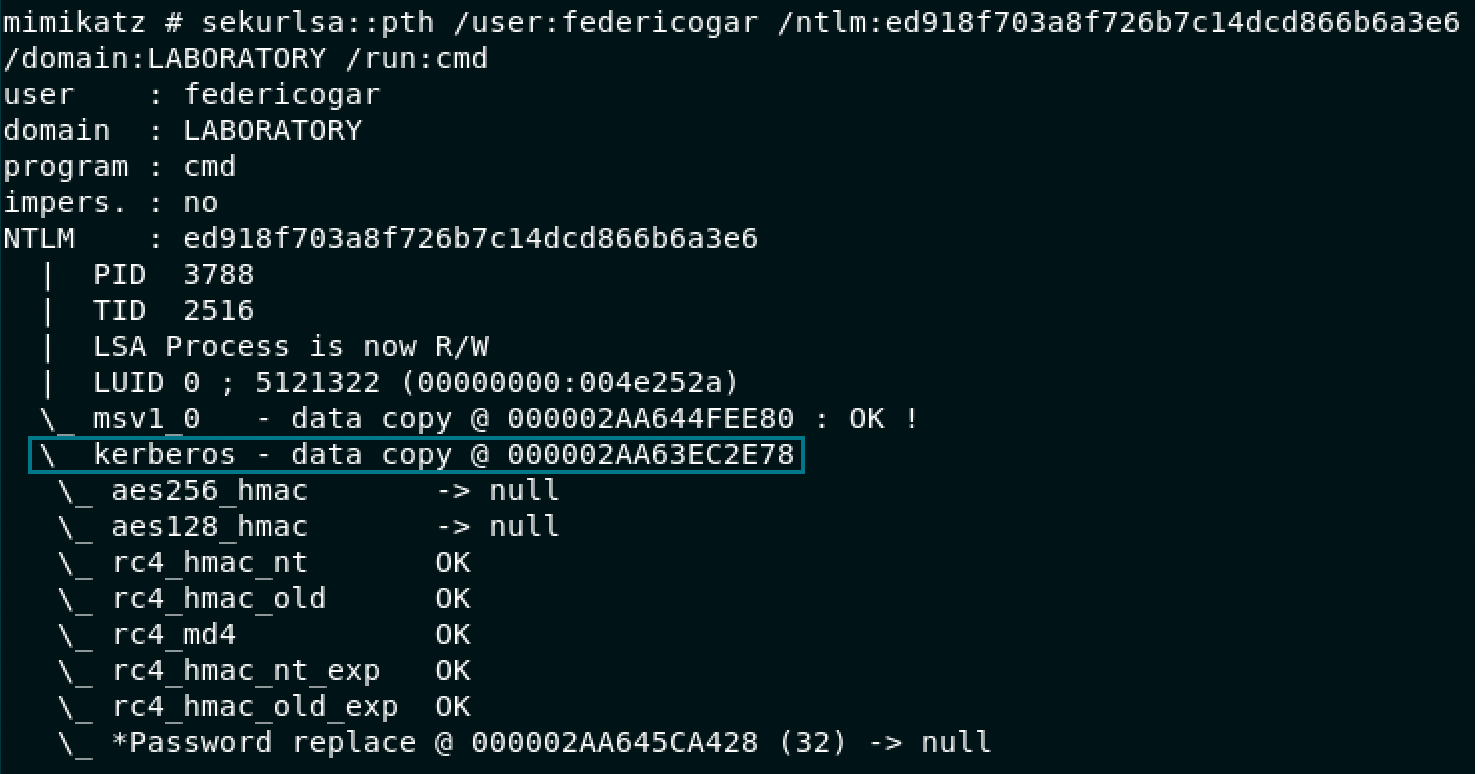
\includegraphics[width=15cm]{OTH/OTH5.png}
\end{center}
\caption{Comando para realizar el ataque overpass the hash.}
\label{OTH5}
\end{figure}

\item Se ejecuta el comando especificado en el comando anterior, en este caso un {\it cmd.exe} en el que se puede acceder al directorio (Figura \ref{OTH6}).
\begin{figure}[H] %[ht!] para here [b] para bottom [t] para top
\begin{center}
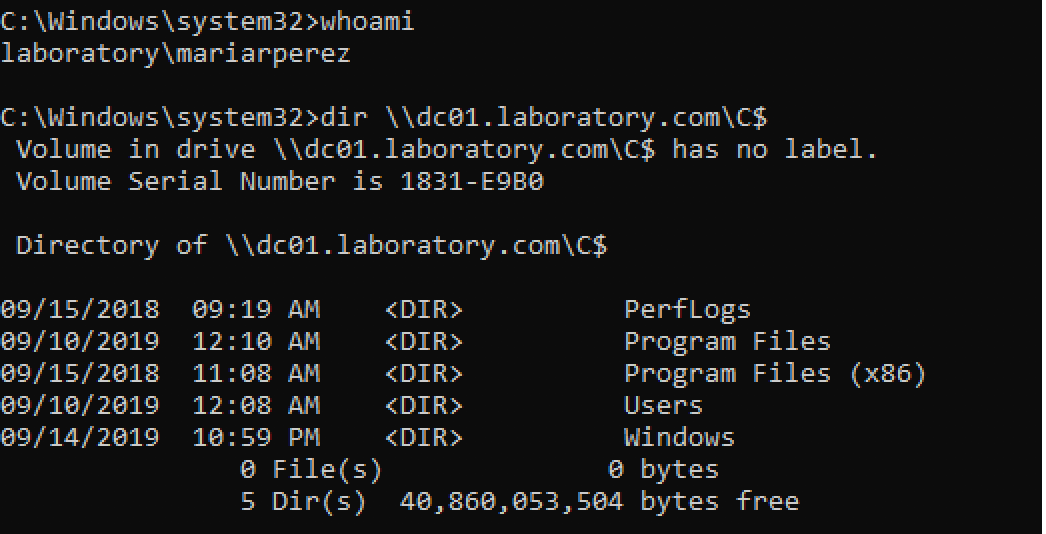
\includegraphics[width=15cm]{OTH/OTH6.png}
\end{center}
\caption{Ataque overpass the hash realizado correctamente.}
\label{OTH6}
\end{figure}

\item En los paquetes KRB5 intercambiados se puede ver que se usa RC4 (Figura \ref{OTH7}) y que la autenticación se completa correctamente recibiendo así un Ticket TGT. 
\begin{figure}[H] %[ht!] para here [b] para bottom [t] para top
\begin{center}
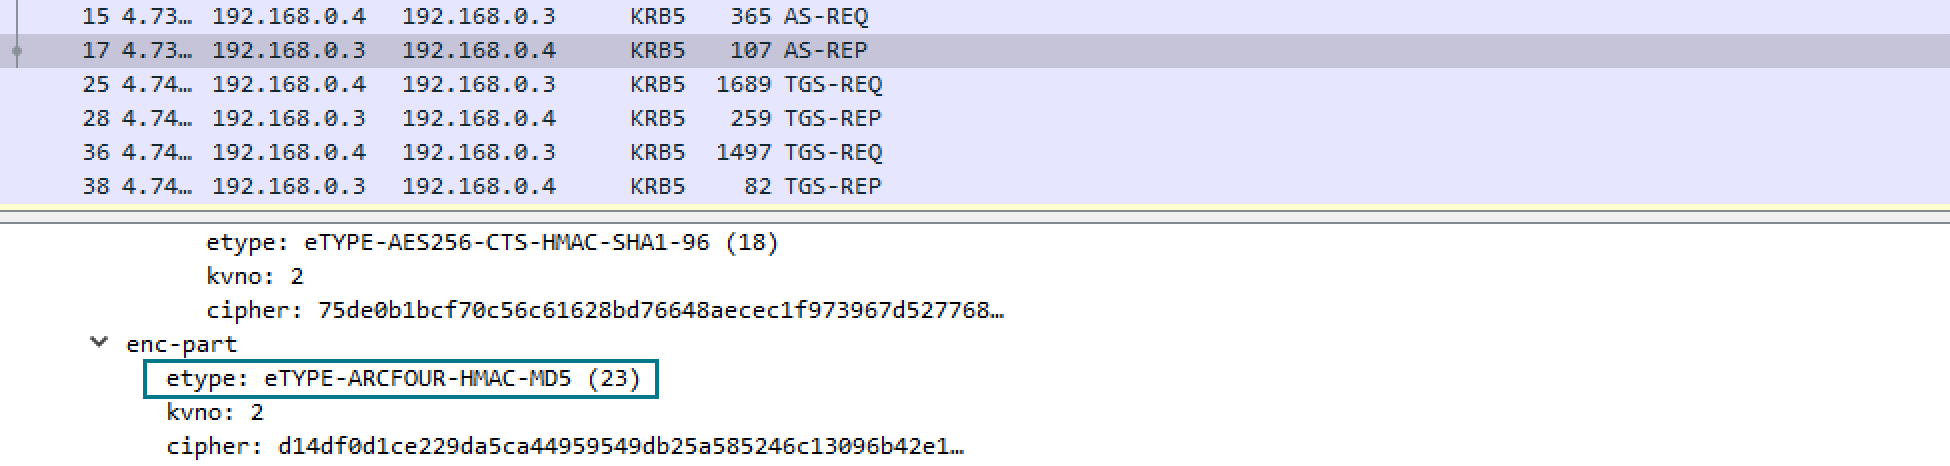
\includegraphics[width=15cm]{OTH/OTH7.png}
\end{center}
\caption{Intercambio de paquetes de Kerberos.}
\label{OTH7}
\end{figure}


\end{enumerate}

\section{Pass The Ticket}

El ataque {\it Pass the ticket}~\cite{Capitulo5:ptt} consiste en la obtención de un Ticket TGS válido de un usuario y la utilización de este para acceder a servicios o recursos donde el usuario tenga acceso. Esta técnica de movimiento lateral y/o movimiento vertical utiliza, para la autenticación de un usario legítimo, un ticket válido encontrado en el sistema. Una característica de este ataque es que no es necesario ser administrador local para importar los tickets de Kerberos.  

\subsubsection{Experimentación}

Para la ejecución del ataque {\it Pass the ticket} es necesario que el usuario con privilegios al que se quiere suplantar haya solicitado un Ticket TGS en la máquina de la que se dispone una conexión activa. A continuación, se detallará el proceso realizado. 

\begin{enumerate}

\item Como se puede observar en la Figura \ref{PTT1}, al igual que en los ataques anteriores, se dispone de una sesión activa a través de una {\it Reverse Shell} interactiva del usuario administrador local {\it mariarperez}. Además, con el comando {\it klist} se pueden listar los tickets tanto TGT como TGS de los que dispone dicho usuario. En este caso no dispone de ninguno.
\begin{figure}[H] %[ht!] para here [b] para bottom [t] para top
\begin{center}
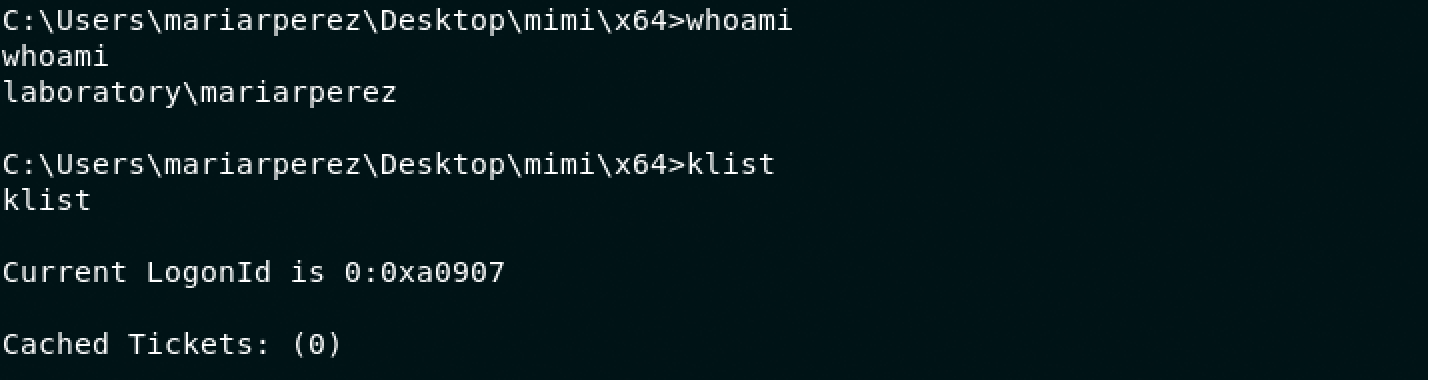
\includegraphics[width=15cm]{PTT/PTT1.png}
\end{center}
\caption{Tickets del usuario mariarperez.}
\label{PTT1}
\end{figure}

\item A través de la herramienta Mimikatz, y ejecuntando el siguiente comando, se obtienen todos los tickets válidos disponibles en el sistema (Figura \ref{PTT2}). Este comando creará un fichero {\it *.kirbi} por cada ticket que haya encontrado. 
\begin{listing}[style=consola, numbers=none]
# sekurlsa::tickets /export
\end{listing}
\begin{figure}[H] %[ht!] para here [b] para bottom [t] para top
\begin{center}
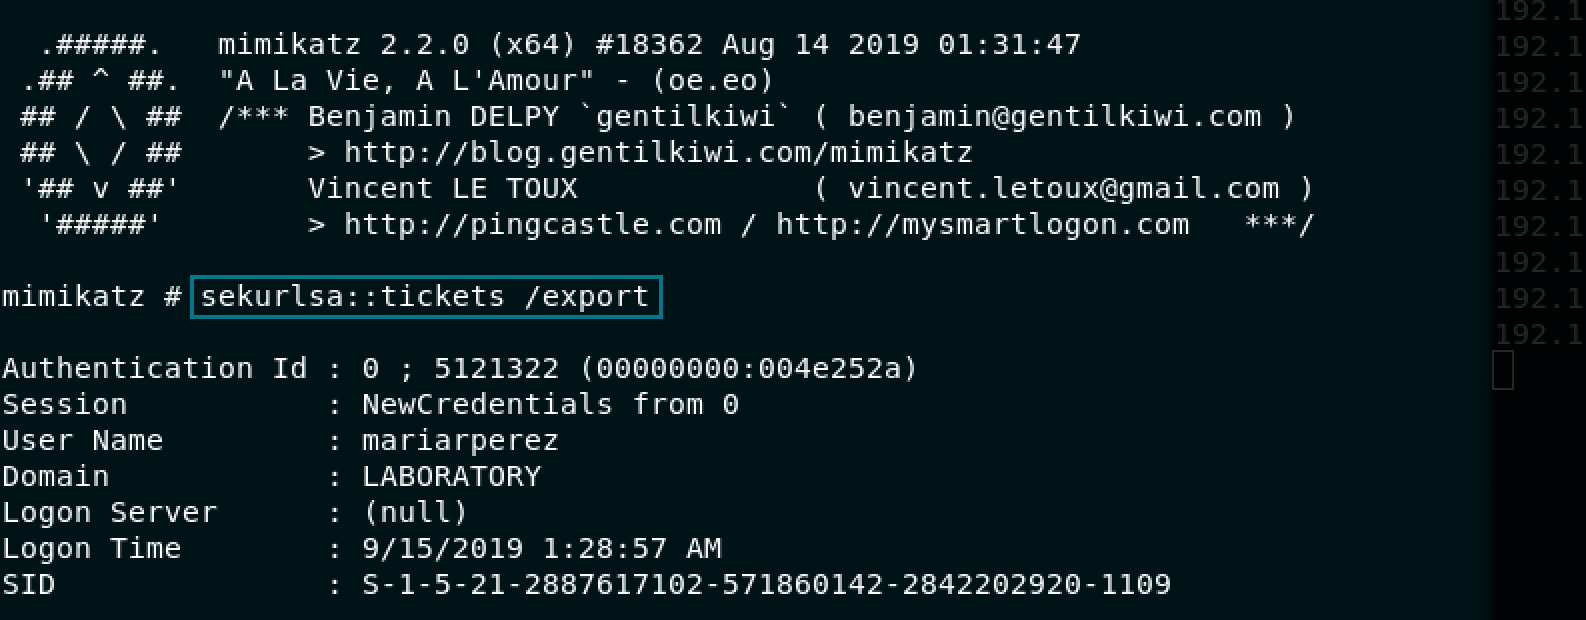
\includegraphics[width=15cm]{PTT/PTT2.png}
\end{center}
\caption{Extracción de tickets a través de Mimikatz.}
\label{PTT2}
\end{figure}

\item Si listamos todos los tickets que ha logrado obtener el comando anterior (Figura \ref{PTT3}) se puede observar que existen tickets cuyo usuario es {\it federicogar}, domain admin de Active Directory. 
\begin{figure}[H] %[ht!] para here [b] para bottom [t] para top
\begin{center}
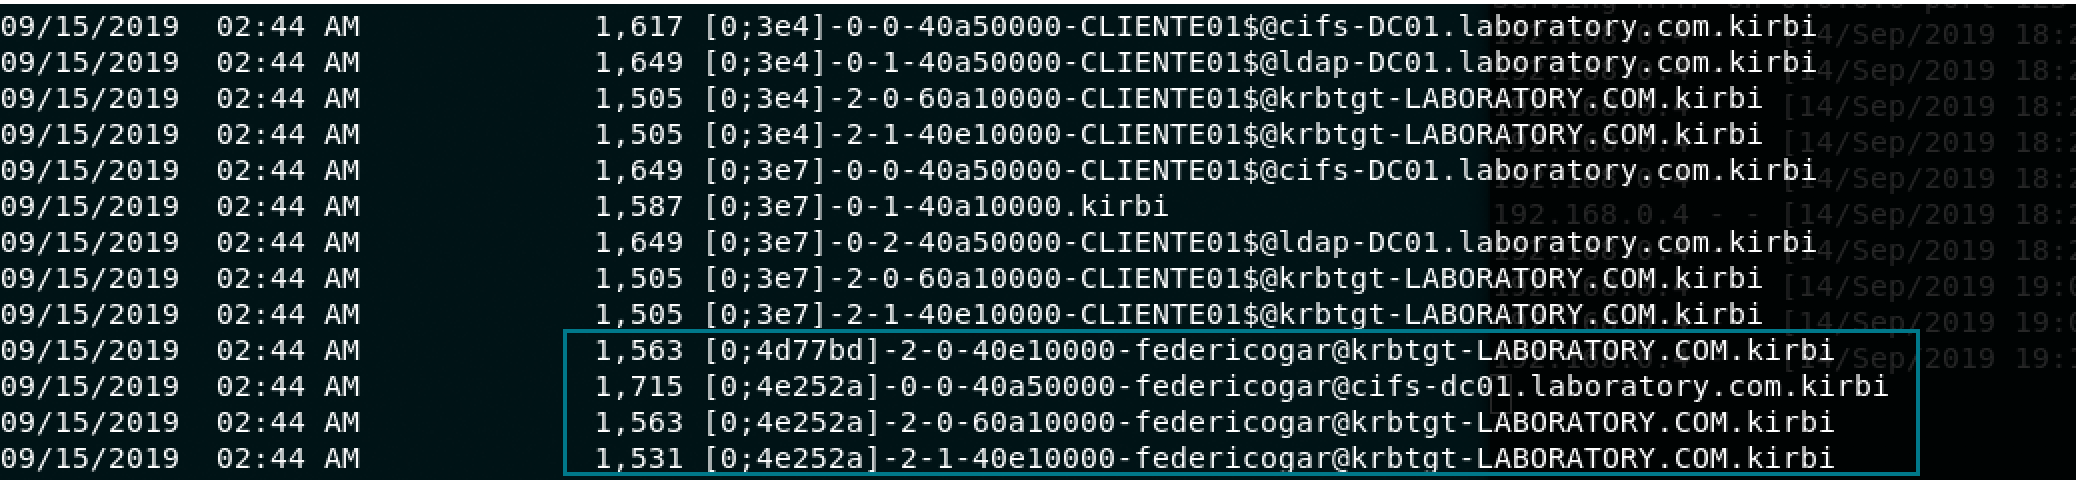
\includegraphics[width=15cm]{PTT/PTT3.png}
\end{center}
\caption{Lista de tickets obtenidos.}
\label{PTT3}
\end{figure}

\item Una vez elegido el ticket, se utiliza de nuevo la herramienta Mimikatz para realizar el ataque de {\it Pass the ticket} a través del comando que se puede ver en la Figura \ref{PTT4}. Para comprobar que el ataque se ha creado correctamente se vuelven a listar los tickets para el usuario {\it mariarperez} y se observa que existe un ticket TGT cuyo cliente es {\it federicogar}.
\begin{figure}[H] %[ht!] para here [b] para bottom [t] para top
\begin{center}
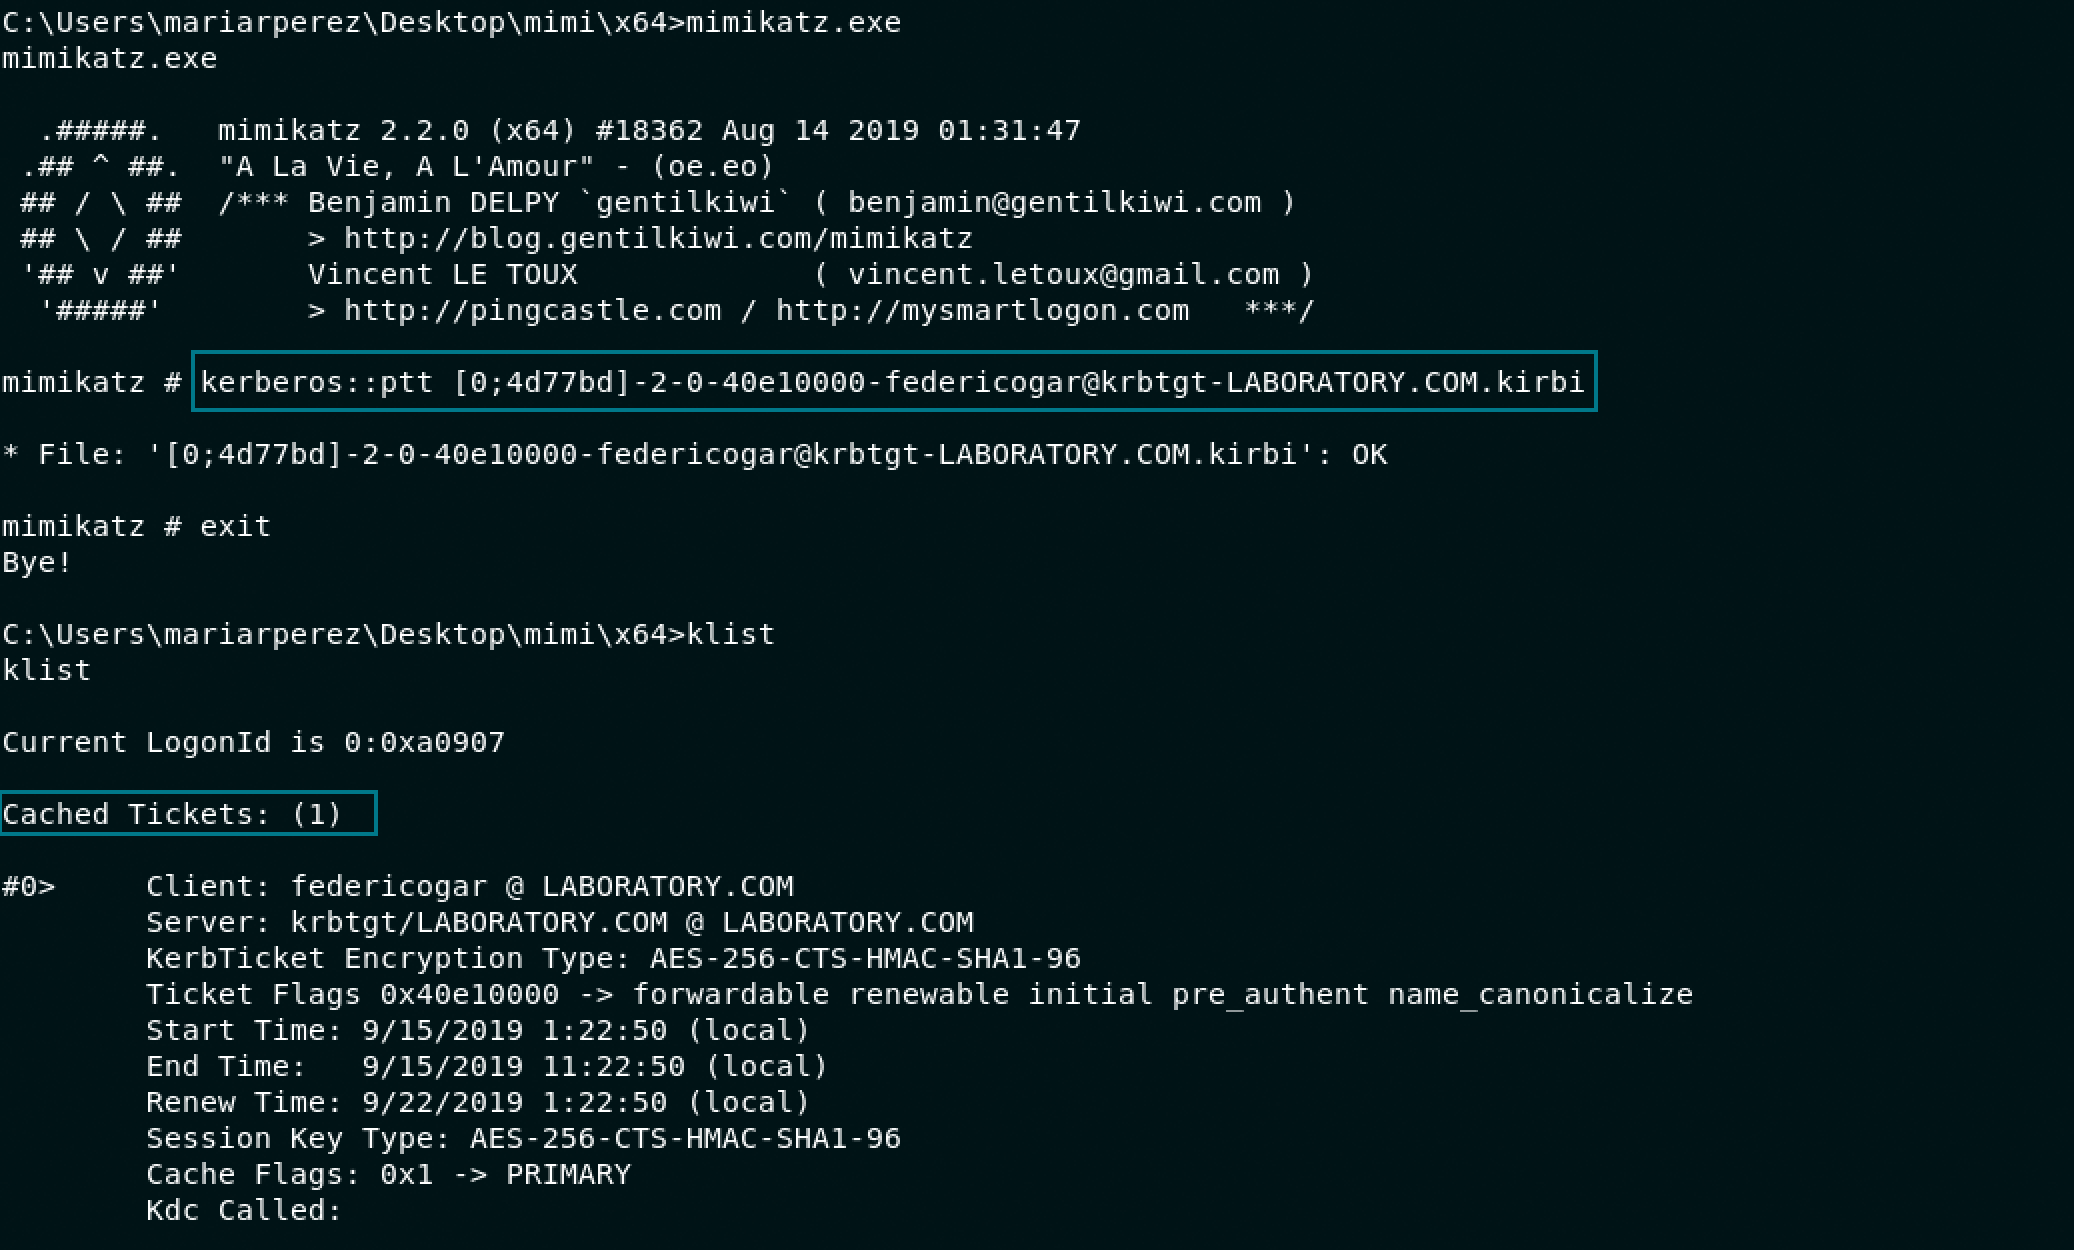
\includegraphics[width=15cm]{PTT/PTT4.png}
\end{center}
\caption{Ataque pass the ticket.}
\label{PTT4}
\end{figure}

\item Con el ticket TGT válido, ya se puede obtener un ticket TGS que permita acceder a los recursos del usuario suplantado (Figura \ref{PTT5}).
\begin{figure}[H] %[ht!] para here [b] para bottom [t] para top
\begin{center}
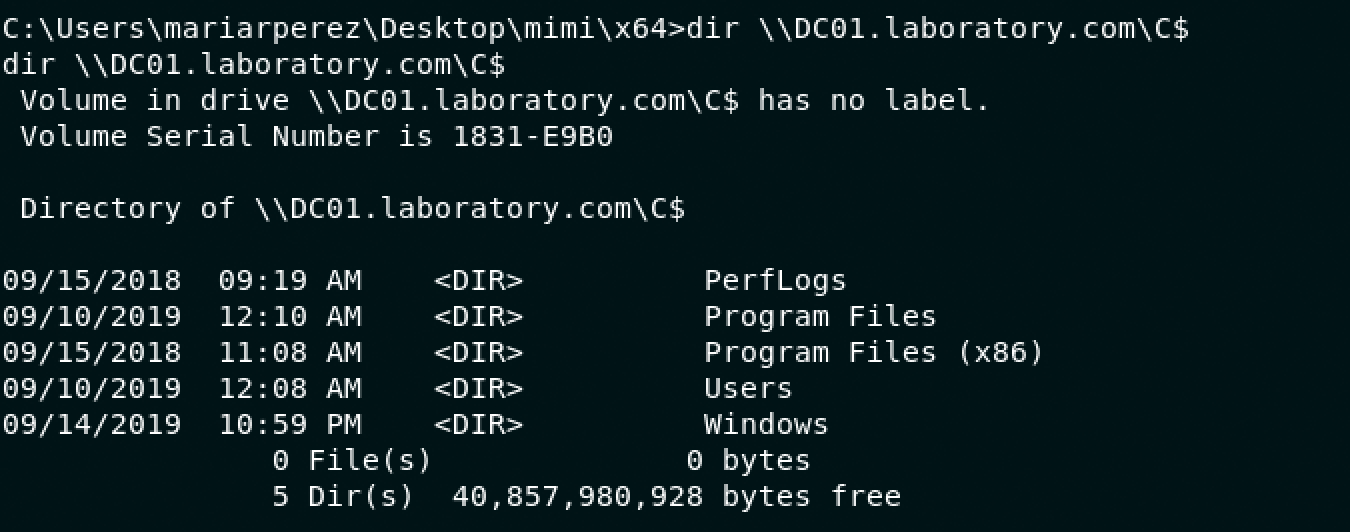
\includegraphics[width=15cm]{PTT/PTT5.png}
\end{center}
\caption{Comprobación del ataque pass the ticket.}
\label{PTT5}
\end{figure}

\end{enumerate}

\section{Golden Ticket}

La técnica {\it Golden Ticket}~\cite{Capitulo5:Kerberos} no es un ataque como tal, es una técnica de persistencia que consiste en generar un ticket TGT cuya caducidad puede ser definida por el atacante. Para ello, es necesario disponer del hash de la cuenta de usuario {\it krbtgt} para poder cifrar el ticket correctamente. Esta técnica es una de las técnicas más importantes ya que al disponer del hash de la cuenta {\it krbtgt} es posible suplantar todas las cuentas del Active Directory y otorga al atacante acceso a todos los recursos del dominio además de ser una técnica prácticamente indetectable ~\cite{Capitulo5:Golden}.

\subsubsection{Experimentación}

Antes de realizar este ataque, como requisito fundamental es necesario obtener el Hash NT o culaquier hash de la cuenta {\it krbtgt}, por lo tanto, es una técnica de post-explotación y persistencia ya que es necesario haber comprometido el Active Directory y disponer de una cuenta {\it Domain Admin}. \\

Para obtener la información de la cuenta {\it krbtgt}, desde el Domain Controller y de nuevo con la herramienta Mimikatz se utiliza el siguiente comando:
\begin{listing}[style=consola, numbers=none]
# lsadump::lsa /inject /name:krbtgt
\end{listing}

Y se obtiene la información de la Figura \ref{GT1}, donde se incluye el Hash NT, el Hash aes256\_hmac y el Hash aes128\_hmac entre otra información. 

\begin{figure}[H] %[ht!] para here [b] para bottom [t] para top
\begin{center}
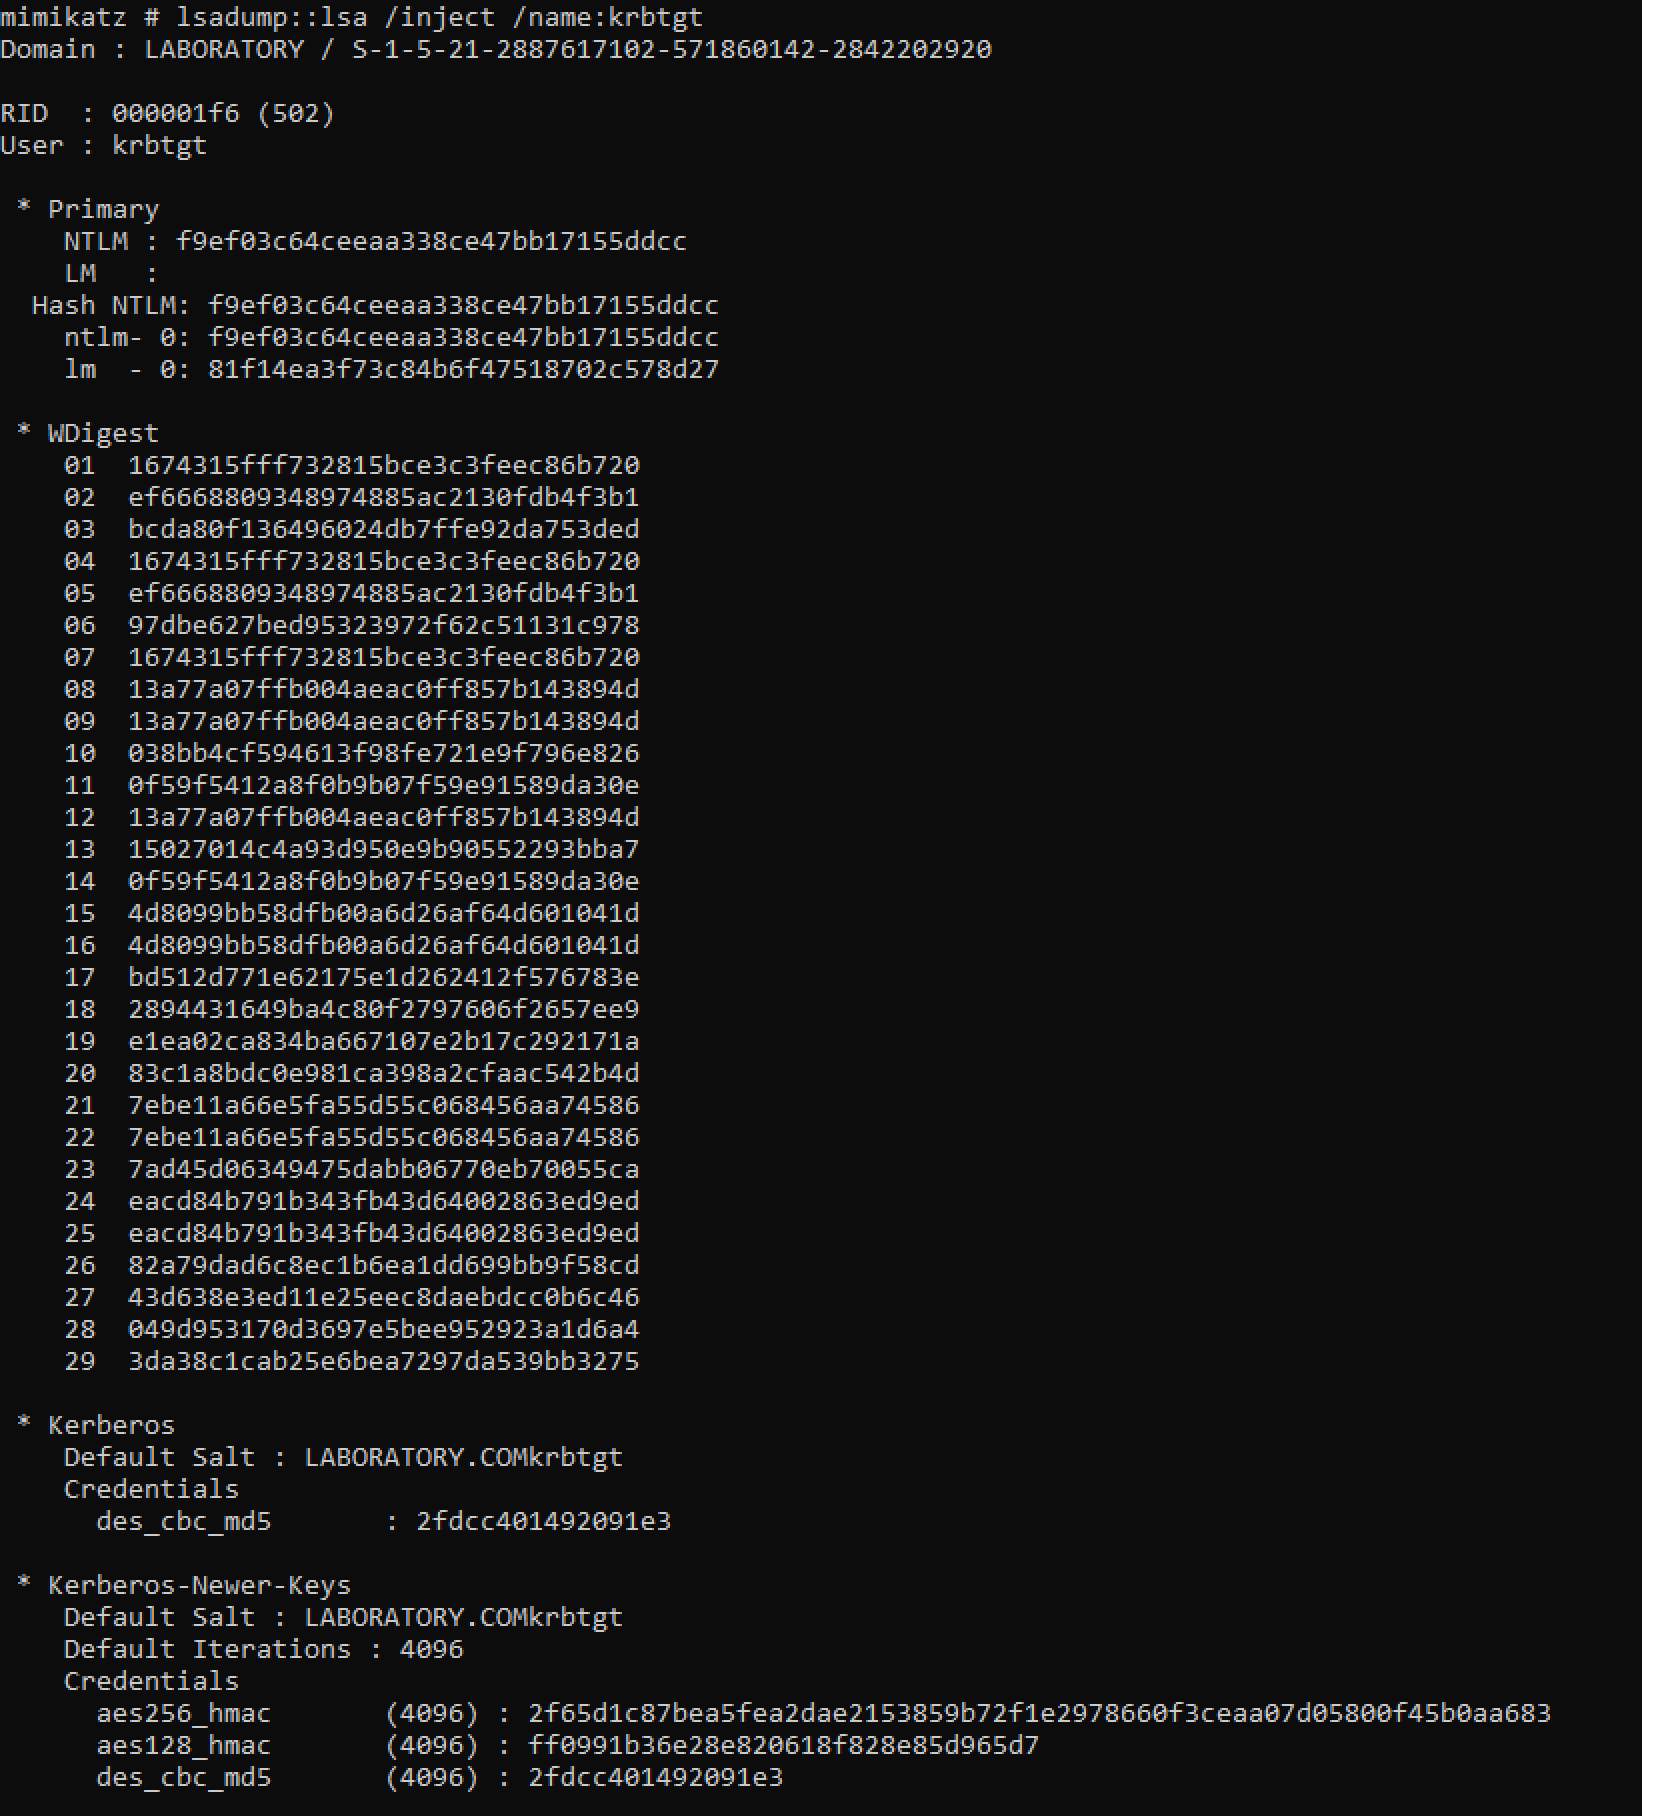
\includegraphics[width=15cm]{GT/GT1.png}
\end{center}
\caption{Obtención de la información de la cuenta krbtgt.}
\label{GT1}
\end{figure}


\begin{enumerate}

\item Una vez obtenido el Hash de la cuenta {\it krbtgt}, desde una cuenta sin privilegios ni tickets asociados (Figura \ref{GT2}) se puede crear un {\it Golden Ticket}. 
\begin{figure}[H] %[ht!] para here [b] para bottom [t] para top
\begin{center}
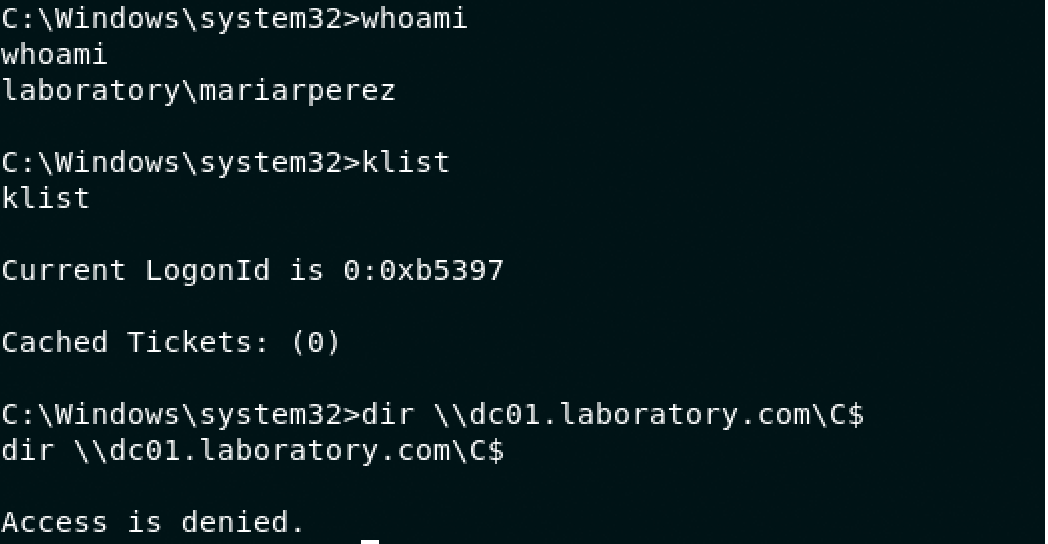
\includegraphics[width=15cm]{GT/GT2.png}
\end{center}
\caption{Cuenta desde la que se va a realizar el ataque.}
\label{GT2}
\end{figure}

\item Para crear un {\it Golden Ticket}, se puede realizar a través de la herramienta Mimikatz. Como se puede ver el Figura \ref{GT3} se ha creado el ticket para el usuario {\it Administrator} cuyo SID corresponde con el del dominio y ha sido obtenido previamente con el comando {\it whoami /user} eliminando la parte correspondiente al ID, aunque llegados a este punto es posible suplantar cualquier cuenta de dominio. Un aspecto a tener en cuenta es la duración de los tickets TGT. Por defecto, los tickets creados le\-gí\-ti\-ma\-men\-te tienen una duración de 10 horas a partir del momento de su creación. Cuando se crea un {\it Golden Ticket} la duración por defecto es de 10 años. Este dato puede hacer saltar los antivirus o incluso que el ticket sea invalidado. Para ello es conveniente indicar la duración del ticket a través de la opción {\it /endin:600}. 

\begin{listing}[style=consola, numbers=none]
# kerberos::golden /domain:[Dominio] /sid:[SID del dominio] /[rc4/aes128/aes256]:[Hash krbtgt] /user:[Usuario a suplantar] /ptt /id:[ID] /groups:[Lista de grupos a los que va a pertenecer el usuario] /endin:600
\end{listing}

\begin{figure}[H] %[ht!] para here [b] para bottom [t] para top
\begin{center}
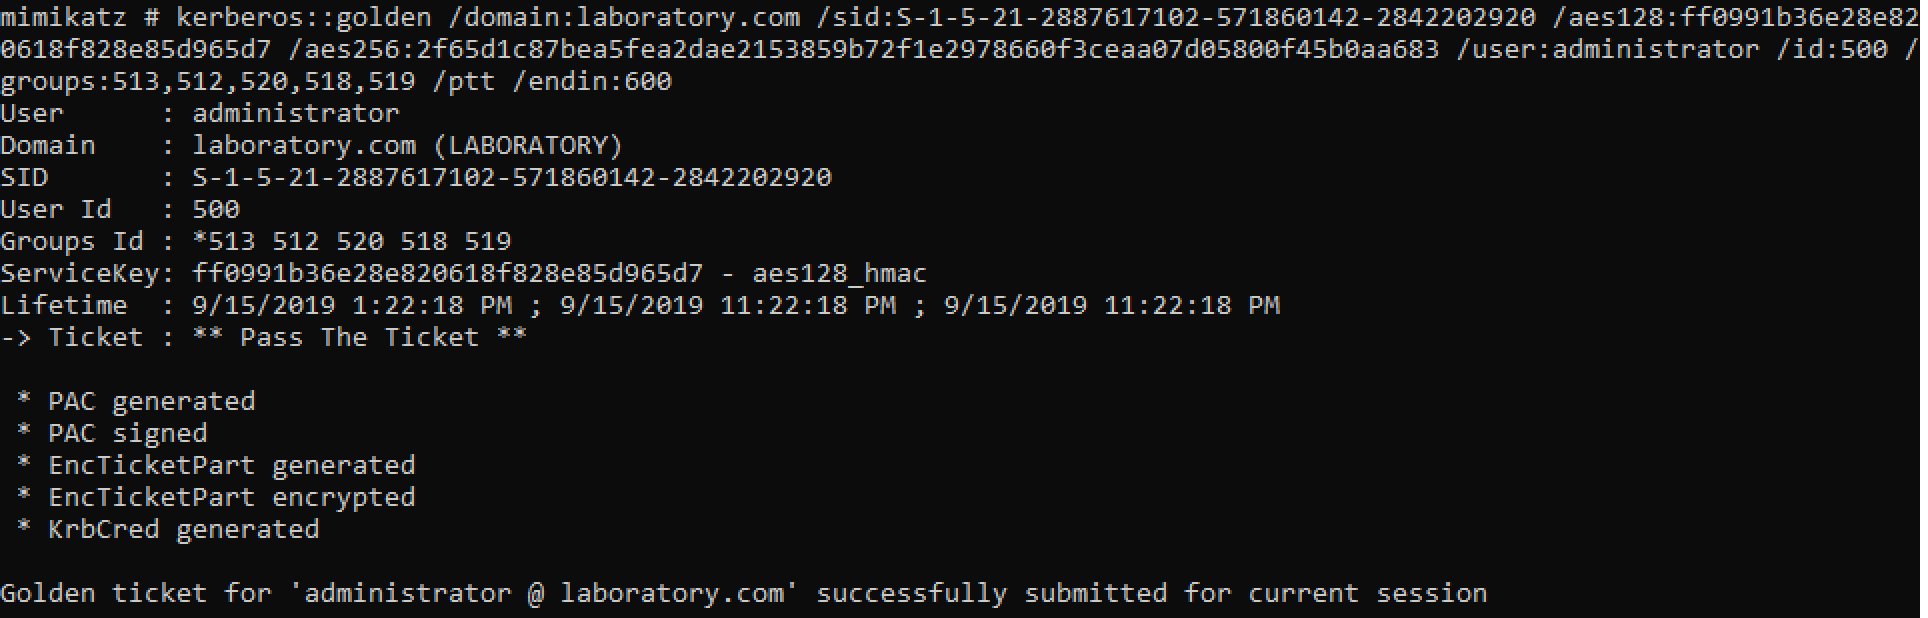
\includegraphics[width=15cm]{GT/GT3.png}
\end{center}
\caption{Creación de un golden ticket.}
\label{GT3}
\end{figure}

\item Por último, se comprueba que el {\it Golden Ticket} se ha creado correctamente (Figura \ref{GT4}) y que se tiene acceso a los ficheros del Domain Controller.
\begin{figure}[H] %[ht!] para here [b] para bottom [t] para top
\begin{center}
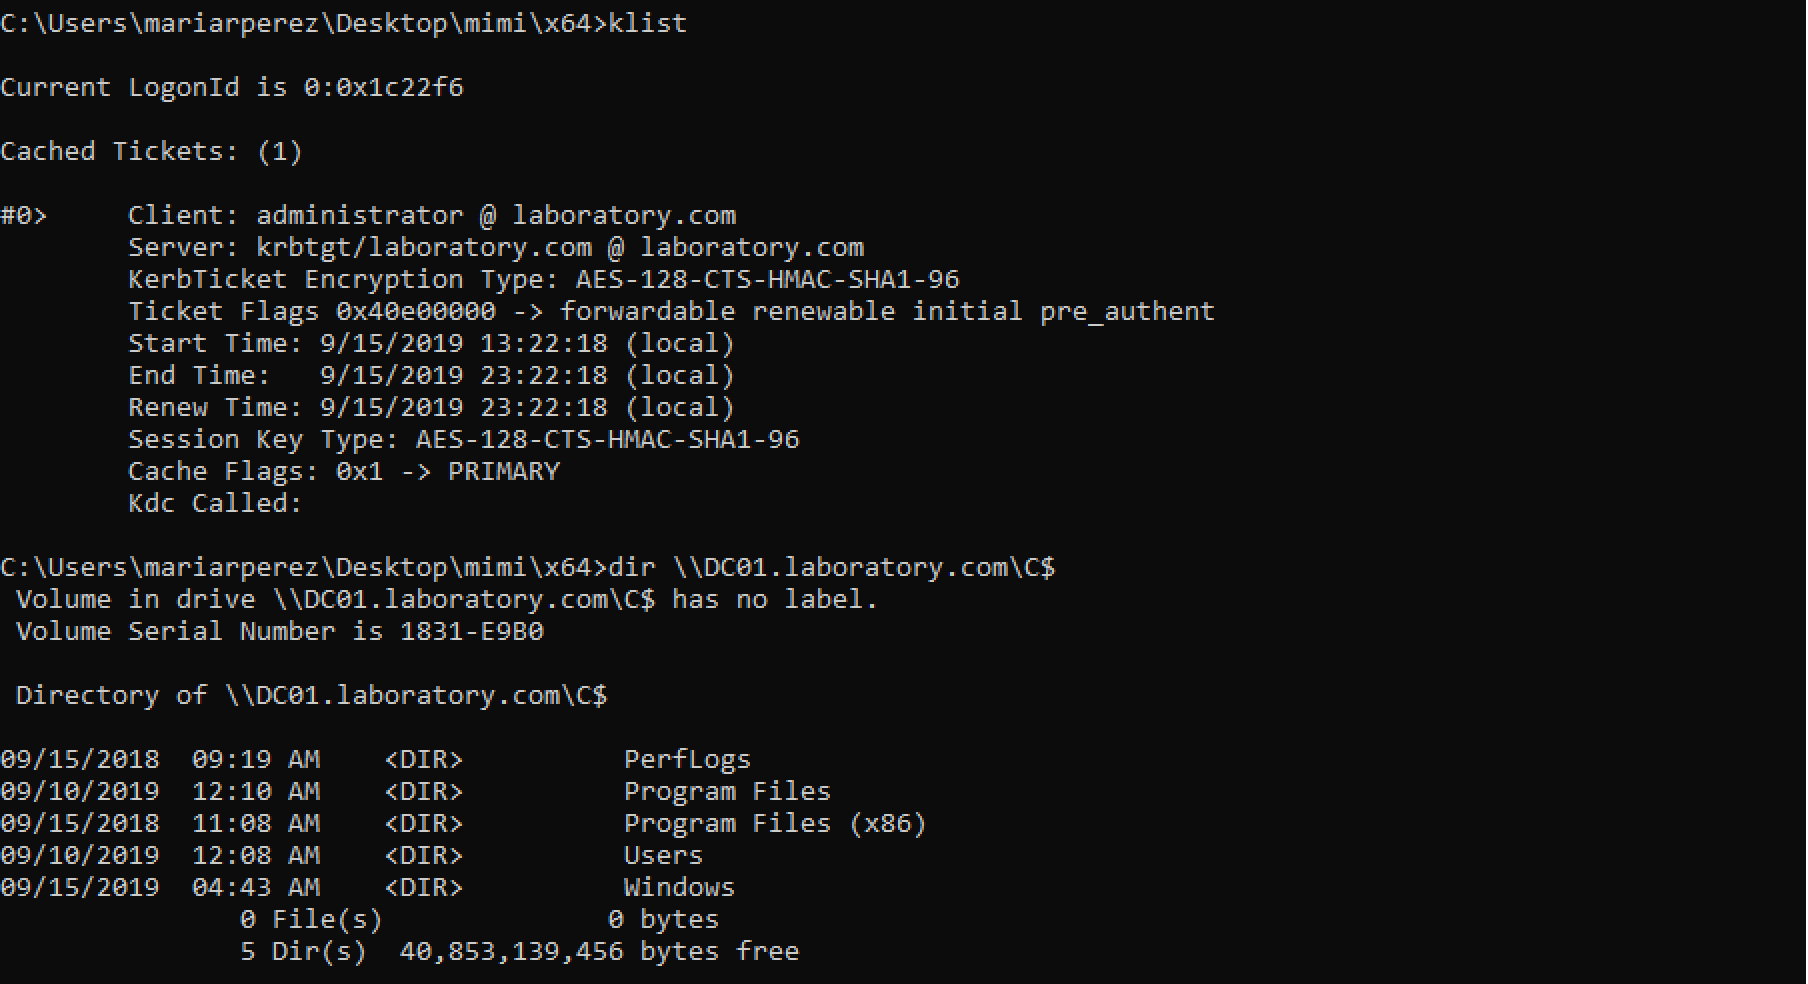
\includegraphics[width=15cm]{GT/GT4.png}
\end{center}
\caption{Golden ticket creado correctamente.}
\label{GT4}
\end{figure}

\end{enumerate}

\section{Kerberoast}

La último técnica contra Active Directory es el ataque {\it Kerberoast}. La idea principal de este ataque es obtener tickets TGS y crackearlos de manera local para obtener la contraseña del servicio o usuario en cuestión. Este es uno de los ataques más utilizados ya que no es necesario una interacción completa con el sistema. El atacante puede pedir un ticket TGS de manera legítima, sin realizar ningún tipo de ataque o usando algún tipo de herramienta de auditoría y crackearlo de manera local en una máquina ajena al dominio. Este ataque aprovecha que los tickets de servicio o tickets TGS están cifrados con el Hash NT de la cuenta del servicio y tiene más probabilidades de que la contraseña sea débil o fácil de obtener. Esta técnica utiliza los Service Principal Name (SPN)~\cite{Capitulo4:SPN} definidos en la sección anterior. 

\subsubsection{Experimentación}

Para poderla llevar acabo en el laboratorio, es necesario añadir a un usuario el atributo SPN, para ello se realizan los siguientes pasos:

\begin{enumerate}

\item Desde el Domain Controller, en la opción de {\it Active Directory Users and Computers} en la pestaña {\it View} se añade la opción de {\it Advanced Features} (Figura \ref{Kerberoast1}). Esto permite que se puedan editar los atributos de un usuario. 
\begin{figure}[H] %[ht!] para here [b] para bottom [t] para top
\begin{center}
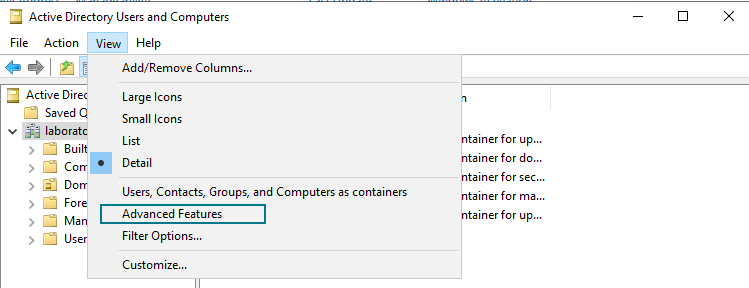
\includegraphics[width=15cm]{Kerberoast/Kerberoast1.png}
\end{center}
\caption{Advanced features.}
\label{Kerberoast1}
\end{figure}

\item Se elige el usuario y se pueden ver las propiedades de este. En la pestaña {\it Attribute Editor} se busca el atributo {\it servicePrincipalName} y se añade el valor que se quiera, en este caso, se ha añadido {\it kerberoast\textbackslash{}testing} como se puede apreciar en la Figura \ref{Kerberoast2}.
\begin{figure}[H] %[ht!] para here [b] para bottom [t] para top
\begin{center}
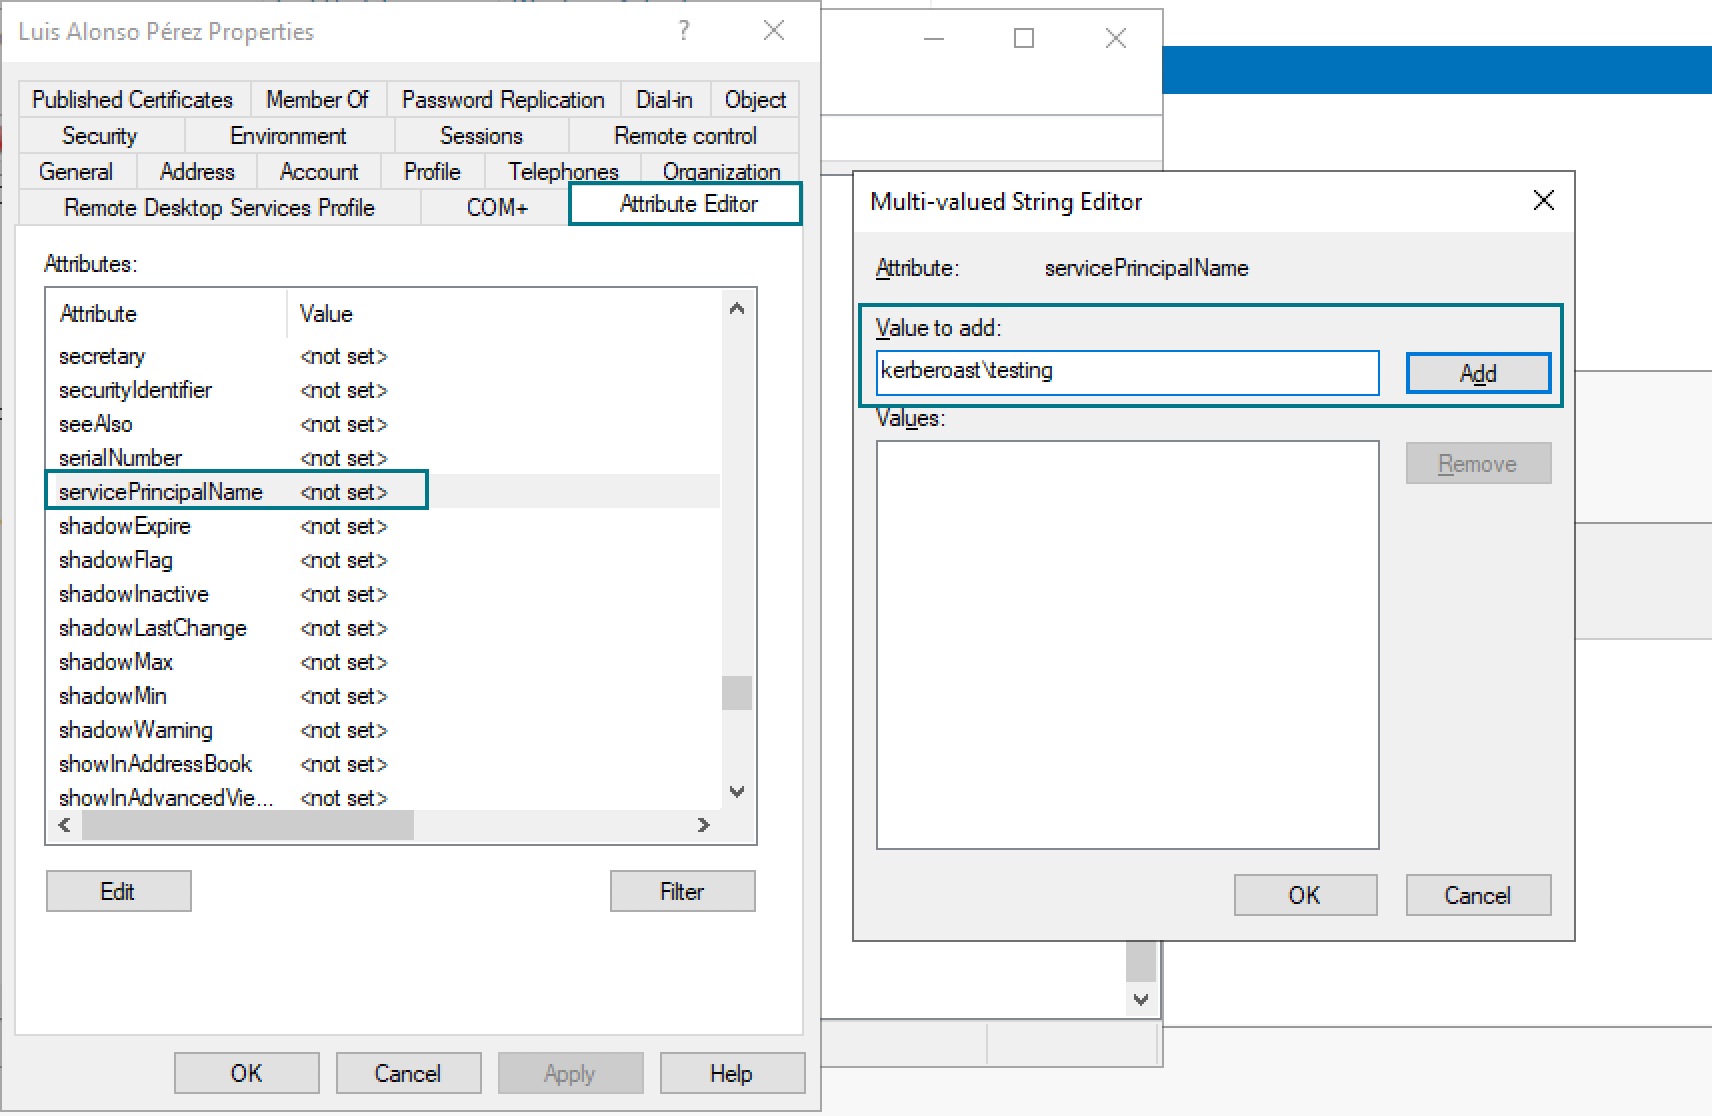
\includegraphics[width=15cm]{Kerberoast/Kerberoast2.png}
\end{center}
\caption{Añadir el atributo SPN al usuario.}
\label{Kerberoast2}
\end{figure}

\end{enumerate}

Después de realizar este cambio, ya se puede realizar el ataque Kerberoast~\cite{Capitulo5:Kerberoast} en el laboratorio creado: 

\begin{enumerate}
\item En primer lugar, a través de la herramienta proporcionada por Microsoft {\it Setspn}, se listan todos los SPN disponibles en el dominio. Como se puede ver en la Figura \ref{Kerberoast3} aparece el SPN creado anteriormente. El comando ejecutado es el siguiente: 

\begin{listing}[style=consola, numbers=none]
# Setspn -T [Dominio] -Q */*
\end{listing}

\begin{figure}[H] %[ht!] para here [b] para bottom [t] para top
\begin{center}
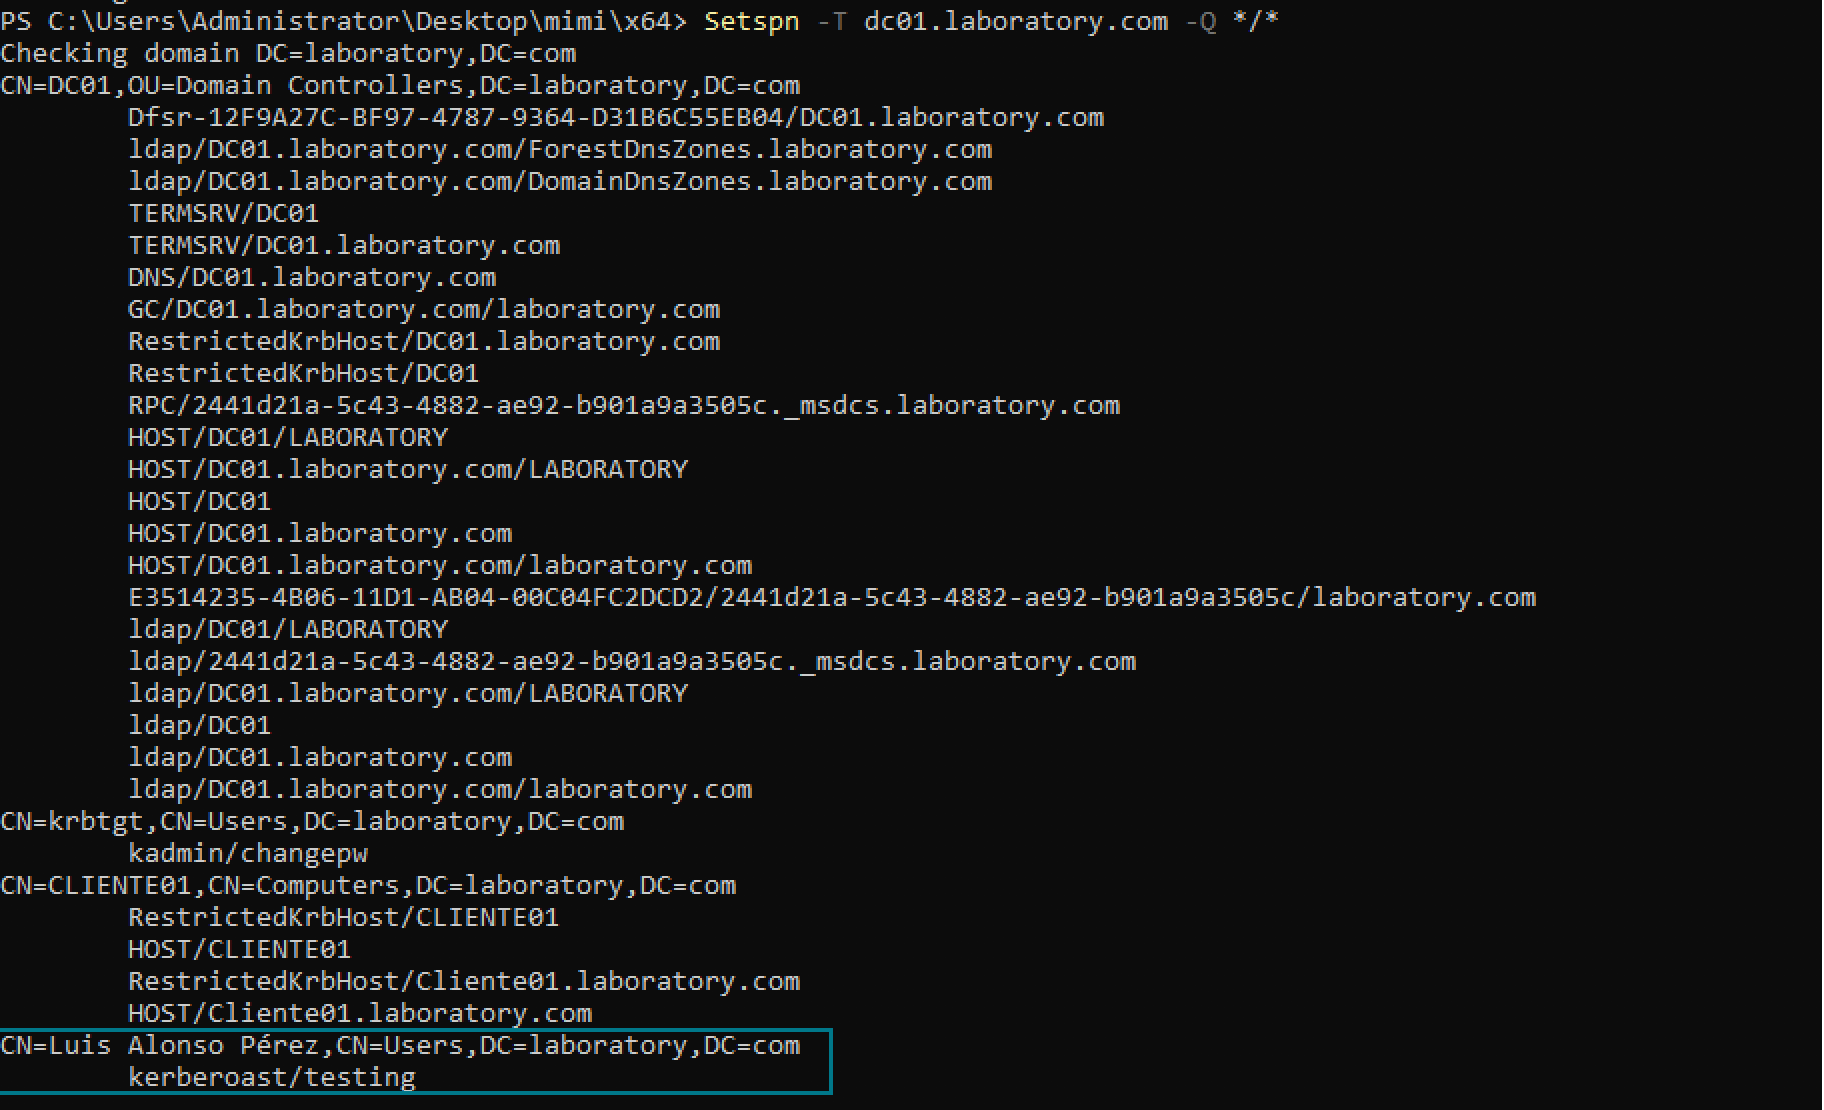
\includegraphics[width=15cm]{Kerberoast/Kerberoast3.png}
\end{center}
\caption{Lista de los SPN disponibles en el dominio.}
\label{Kerberoast3}
\end{figure}

\item Posteriormente, se solicita un ticket TGS para la SPN {\it kerberoast\textbackslash{}testing} (Figura \ref{Kerberoast4}) a través de los siguientes comandos:

\begin{listing}[style=consola, numbers=none]
# Add-Type -AssemblyName System.IdentityModel
# New-Object System.IdentityModel.Tokens.KerberosRequestorSecurityToken -ArgumentList "kerberoast/testing"
\end{listing}

\begin{figure}[H] %[ht!] para here [b] para bottom [t] para top
\begin{center}
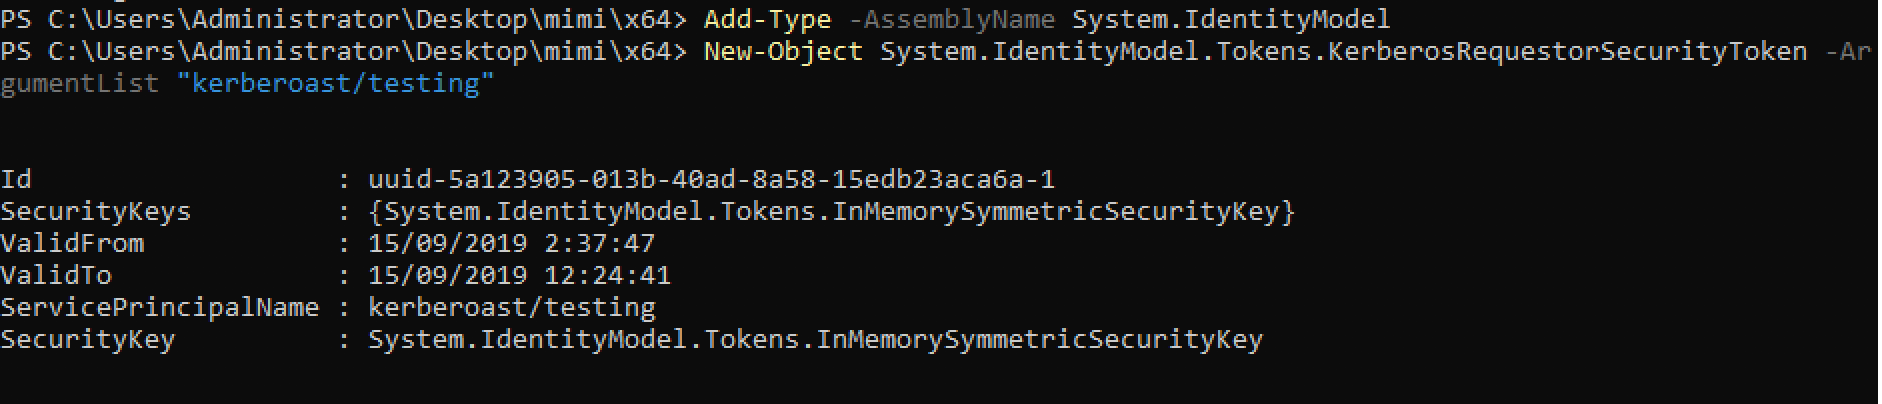
\includegraphics[width=15cm]{Kerberoast/Kerberoast4.png}
\end{center}
\caption{Solicitud de TGS.}
\label{Kerberoast4}
\end{figure}

\item Una vez creado el TGS, se exporta con la herramienta Mimikatz (Figura \ref{Kerberoast5}) a través del siguiente comando:
\begin{listing}[style=consola, numbers=none]
# kerberos::list /export
\end{listing}
\begin{figure}[H] %[ht!] para here [b] para bottom [t] para top
\begin{center}
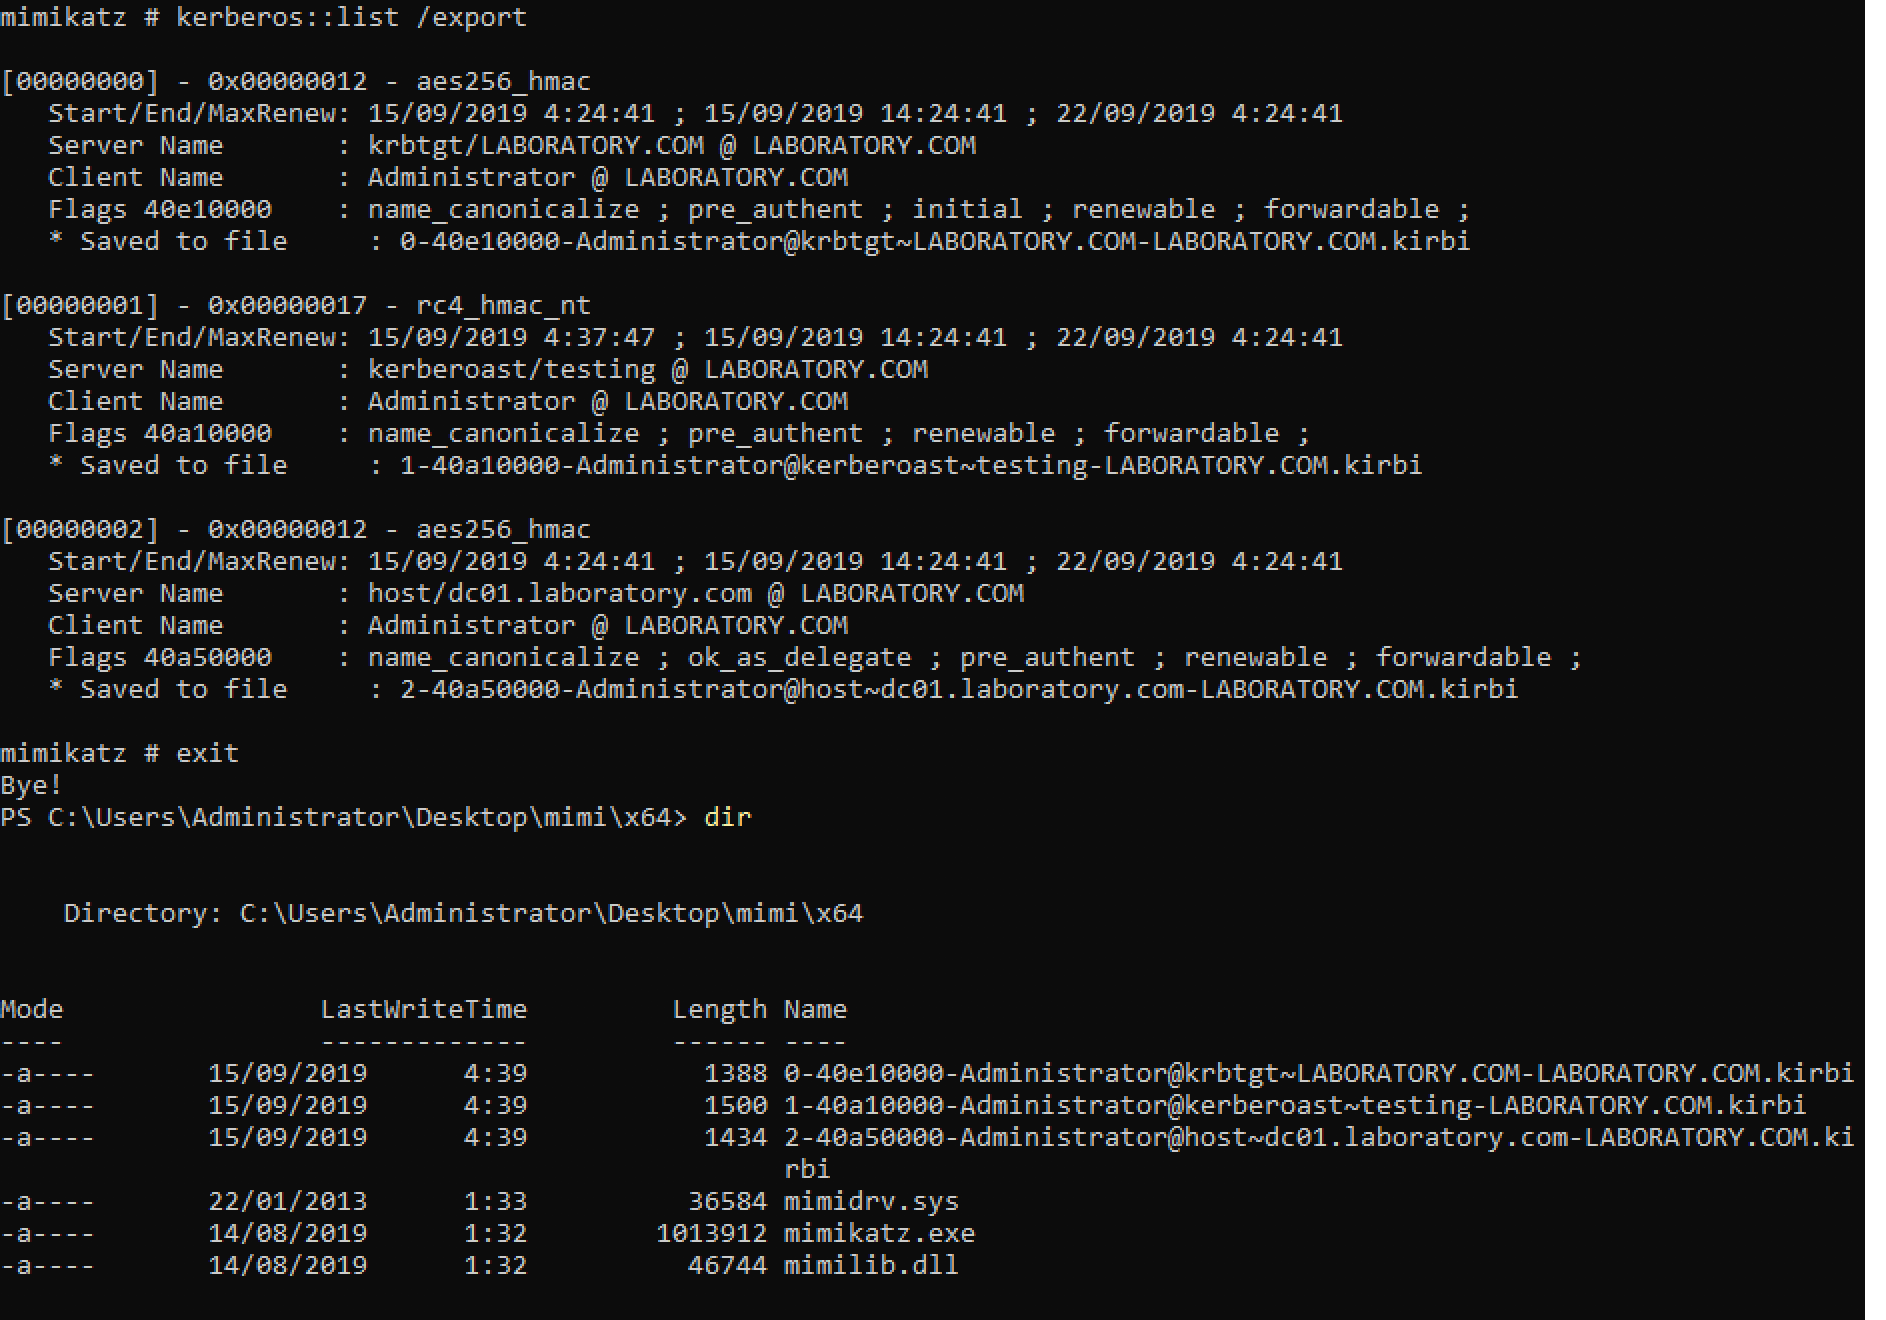
\includegraphics[width=15cm]{Kerberoast/Kerberoast5.png}
\end{center}
\caption{Expotar los tickets TGS.}
\label{Kerberoast5}
\end{figure}

\item Se exfiltra el ticket TGS creado anteriormente, se crackea con la herramienta {\it tgsrepcrack.py} en una máquina ajena al dominio y se obtiene la contraseña en texto plano (Figura \ref{Kerberoast6}). 
\begin{figure}[H] %[ht!] para here [b] para bottom [t] para top
\begin{center}
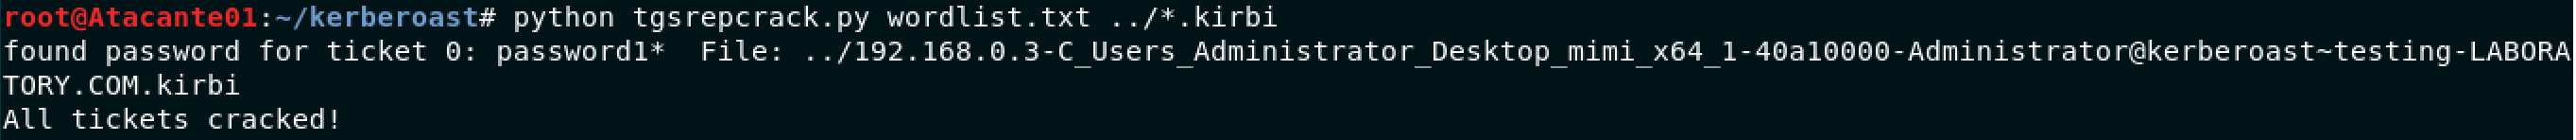
\includegraphics[width=15cm]{Kerberoast/Kerberoast6.png}
\end{center}
\caption{Cracking del ticket TGS.}
\label{Kerberoast6}
\end{figure}

\end{enumerate}
